% STATUS: reviewed
\chapter{Atitikties programos dokumentai}\label{ch:programme}

Atitikties ataskaita parodo, kokia yra įmonės padėtis teisės požiūriu. Tačiau atitikties
valdymo sistemai reikia ir savų dokumentų: politikos, atsakomybių paskirstymo, teisinės
rizikos vertinimo. Sistema iš įmonės dokumentų rinkinio parengia trijų tokių dokumentų
projektus, kodu patikrina, ar kiekvienas projektas laikosi nustatytų taisyklių, o redaguoti ir
tvirtinti palieka žmogui. Šiame skyriuje aprašoma, kokie tai dokumentai, kaip vienas iš jų
generuojamas, ko klausia šešios juos parengiančios instrukcijos, kokių taisyklių atsakymams
reikalauja kodas, kaip apskaičiuojami teisinės rizikos registro skaičiai ir ką su projektu
toliau gali daryti žmogus, eksportas ir pokalbių asistentas. Skyrius baigiamas tuo, kiek
kainuoja vienas generavimas, ir aiškiu pasakymu, kaip šios instrukcijos matuojamos ir kaip
ne.


% ------------------------------------------------------------
\section{Kas yra programos dokumentas}\label{sec:programme:what}

\term{Programos dokumentas} --- tai vienas įmonės atitikties programos dokumentas, viena jo
versija: modelio parengtas turinys, rūšies taisyklės su tuo, kaip turinys jų laikėsi ar jas
pažeidė, įrašas apie tai, ką generavimas skaitė, ir kiek jis kainavo. API programėlė yra
\file{programme/}, lentelė --- \code{work_products} (\cref{ch:data}). Yra trys \term{rūšys}, ir
tai būtent tie dokumentai, kurių reikalauja antroji ir trečioji kurso užduotys
(\cref{ch:course}).

\begin{table}[H]
\caption{Trys programos dokumentų rūšys (\file{programme/kinds.py}, \code{KINDS}); pavadinimas --- toks, kokį rodo konsolė}\label{tab:programme:kinds}
\begin{tabularx}{\textwidth}{@{}L{19mm}L{37mm}YL{17mm}@{}}
\toprule
\hd{Rūšis} & \hd{Pavadinimas} & \hd{Ką apima} & \hd{Remiasi} \\
\midrule
\code{policy} & Atitikties politika &
  Aštuonių dalių atitikties politika; prie kiekvienos dalies --- įmonės dokumentų ištraukos,
  kuriomis ji remiasi, jos teisinis pagrindas ir klausimai, paliekami spręsti valdymo organui;
  kiekvienas rinkinio dokumentas, priskirtas dokumentų hierarchijos lygmeniui; 2 ir 3~lygmens
  dokumentai, kurių įmonei dar trūksta. & --- \\
\code{governance} & Valdymo struktūra, atitikties procesas ir RACI &
  Dokumentuose įvardytos pareigybės ir padaliniai; rolės, kurių trūksta arba kurios taip, kaip
  aprašytos, negali veikti; siūloma struktūra kaip medis; atitikties valdymo procesas etapais;
  RACI matrica, kuri kiekvieną etapą paskiria struktūros rolėms. & \code{policy} \\
\code{risks} & Teisinės atitikties rizikos vertinimo kriterijai ir registras &
  Tikimybės ir poveikio kriterijai; penki 5×5 matricos rizikos lygiai ir ką kiekvienas reiškia
  įmonei; rizikos scenarijai su jų balais ir reagavimu --- kartu tai sudaro teisinės rizikos
  registrą. & \code{policy}, \code{governance} \\
\bottomrule
\end{tabularx}
\end{table}

Rūšis --- tai Python modulis su penkiais vardais: \code{TITLE} (kiekvienai kalbai),
\code{NEEDS} (rūšys, kuriomis ji remiasi), \code{STEPS} (jos dviejų modelio iškvietimų,
kaip užduoties etapų, pavadinimai), \code{generate(run)} ir
\code{validate(content, library, language, judge=None)}. Stulpelis \code{kind} neturi jokio
duomenų bazės apribojimo, todėl ketvirtajai rūšiai prireiktų modulio, jo instrukcijų ir
puslapio konsolėje, bet ne migracijos.

\paragraph{Ką rūšis gauna iš kitų.} \code{NEEDS} įvardija ankstesnes rūšis; generavimas
kiekvienos iš jų ieško kaip įmonės patvirtintos versijos su didžiausiu numeriu, o kai
patvirtintos nėra --- kaip naujausio projekto (\code{Run.__init__} faile
\file{programme/run.py}). Rūšį galima generuoti ir be jų: tada instrukcijai pasakoma, kad tokio
dokumento nėra. Perduodama nedaug ir tiksliai (\cref{fig:programme:builds}). Valdymo struktūros
instrukcijos gauna tris politikos dalis --- \code{mandate}, \code{roles} ir \code{processes},
kiekvieną sutrumpintą iki 1\,800 ženklų --- kartu su politikos versija ir žinia, ar ji
patvirtinta. Rizikos scenarijų instrukcija gauna valdymo struktūros mazgų, kurių rūšis yra
\code{unit} arba \code{function}, pavadinimus. Politika nurodoma tarp dokumentų, kuriais
registras remiasi, ir įrašoma į jo \code{basis}, tačiau jos tekstas neperduodamas nė vienai iš
dviejų rizikos instrukcijų. Be to, kiekviena rūšis skaito naujausią įmonės ataskaitą, kurios
būsena yra \code{done}, nesvarbu, ar ji patvirtinta, ar ne (\cref{sec:programme:report}).

\begin{figure}[H]
\centering
\begin{tikzpicture}[node distance=11mm and 10mm]
  \node[svc, text width=56mm] (policy) {\textbf{policy}\\ {\scriptsize aštuonios dalys · dokumentų hierarchija · trūkstami dokumentai}};
  \node[svc, text width=56mm, below=of policy] (gov) {\textbf{governance}\\ {\scriptsize pareigybės ir spragos · struktūra · procesas · RACI matrica}};
  \node[svc, text width=56mm, below=of gov] (risks) {\textbf{risks}\\ {\scriptsize kriterijai · apetitas · scenarijai (registras)}};
  \node[store, text width=27mm, left=of gov] (lib) {įmonės profilis ir dokumentų rinkinys};
  \node[data, text width=24mm, right=of gov] (report) {naujausia baigta ataskaita};
  \draw[flow] (policy) -- node[lbl, right=1mm] {jos dalys \emph{mandate}, \emph{roles}, \emph{processes}} (gov);
  \draw[flow] (gov) -- node[lbl, right=1mm] {jos struktūros padaliniai ir funkcijos} (risks);
  \draw[flow] (lib.north) |- (policy.west);
  \draw[flow] (lib) -- (gov);
  \draw[flow] (lib.south) |- (risks.west);
  \draw[flow] (report.north) |- (policy.east);
  \draw[flow] (report) -- (gov);
  \draw[flow] (report.south) |- (risks.east);
\end{tikzpicture}
\caption{Iš ko generuojama kiekviena rūšis. Profilis ir visi dokumentai ištisai patenka į abu
kiekvienos rūšies iškvietimus. Ataskaita kiekvieną rūšį pasiekia kaip santrauka: jos teisės
aktai, skaičiai ir atviros temos; registro scenarijai, be to, gauna rimčiausias atviras jos
išvadas.}\label{fig:programme:builds}
\end{figure}

\paragraph{Saugoma eilutė.} \code{work_products} eilutė priklauso įmonei ir rūšiai; ji turi
\code{version}, kuri didėja kiekvienai įmonei ir rūšiai atskirai (unikalumo apribojimas),
\code{language} (\code{lt} arba \code{en}) ir \code{status}: \code{queued}, \code{running},
\code{draft}, \code{approved}, \code{failed} arba \code{cancelled}. Esmę saugo keturi JSON
stulpeliai. \code{content} --- pats dokumentas, kurio forma priklauso nuo rūšies.
\code{checks} --- rūšies taisyklių sąrašas su tuo, kaip turinys paskutinį kartą jų laikėsi ar
jas pažeidė. \code{basis} nurodo, ką generavimas skaitė: ataskaitos id, ankstesnius programos
dokumentus su jų versijomis ir būsenomis ir kiekvieną dokumentą su pavadinimu ir SHA-256
maiša, kad skaitytojas galėtų nustatyti, kuo projektas remiasi. \code{stats} saugo
generavimo žetonus ir kainą bei instrukcijų versijas ir modelius, kurie jį parengė. Eilutėje
taip pat įrašoma, kas ją sukūrė, kas paskutinis redagavo ir kas patvirtino, ir kada.

\begin{humanbox}{Sistema rengia projektą ir tikrina; tvirtina žmogus}
Jokia kodo vieta nenustato programos dokumentui būsenos \code{approved}, išskyrus prisijungusio
naudotojo patvirtinimo užklausą (\code{product_item} faile \file{programme/api/views.py}),
kurią siunčia dokumento puslapis. Kol niekas dokumento nepatvirtina, jis lieka projektas.
Projekto PDF tai nurodo viršelyje --- \enquote{Projektas --- žmogaus dar nepatvirtintas} ---,
o Word failas --- po pavadinimu; Excel darbaknygėje tokios žymos nėra.
\end{humanbox}


% ------------------------------------------------------------
\section{Kaip parengiamas programos dokumentas}\label{sec:programme:generation}

Programos dokumentą generuoja viena foninė užduotis, \code{programme.generate}, keturiais
etapais: perskaitomi dokumentai, du kartus kviečiamas modelis ir patikrinamos atsakymo
nuorodos. Šiame poskyryje generavimas sekamas nuo užklausos iki projekto.

\subsection{Generavimo pradžia}

Naudotojas generavimą pradeda įmonės skiltyje \ui{Programa} mygtuku \ui{Generuoti}, po
dialogo, kuriame nurodoma trukmė ir kaina ir pasirenkama dokumento kalba; generavimą gali
pradėti ir pokalbių asistentas (\cref{sec:programme:chat}). Abu siunčia
\route{POST}{/api/companies/{id}/programme} su rūšimi ir kalba. Rodinys
\code{company_programme} faile \file{programme/api/views.py} į nežinomą rūšį ar kitą kalbą nei
\code{lt} ir \code{en} atsako 400 \code{INVALID_FIELD}, o tinkamą užklausą atmeta dar trimis
atvejais:

\begin{itemize}
  \item įmonė neturi nė vieno dokumento su išgautu tekstu (409 \code{NO_DOCUMENTS}) ---
        programos dokumentas rašomas iš dokumentų rinkinio ir iš nieko kito;
  \item naudotojui liko mažiau nei \code{MIN_BUDGET_TO_START_USD}~=~0,25~\$ šiandienos
        biudžeto (429 \code{BUDGET_EXCEEDED}); naudotojas be dienos limito praeina visada;
  \item tos pačios rūšies dokumentas įmonei jau laukia eilėje arba generuojamas (409
        \code{ALREADY_RUNNING}); patikra ir įterpimas vykdomi užrakinus įmonės eilutę, todėl
        dvi vienu metu atėjusios užklausos negali abi praeiti.
\end{itemize}

Priešingu atveju rodinys sukuria eilutę su kitu versijos numeriu ir būsena \code{queued},
įtraukia užduotį į eilę su duomenimis \code{{product_id}} ir įrašo veiksmų žurnalo įrašą
\code{programme.create}. Naujos versijos generavimas niekada nepaliečia ankstesnių.

\subsection{Keturi etapai ir jų eiga}

Užduoties tvarkyklė yra \code{generate} faile \file{programme/run.py}. Ji sukuria \code{Run}
--- objektą, su kuriuo dirba rūšies modulis --- ir vykdo etapus (\cref{tab:programme:steps}).
Kiekvienas etapas atidaro užduoties etapą (\cref{ch:arch}) ir įrašo į užduotį etapo
pavadinimą ir tai, kurioje generavimo vietoje tas etapas prasideda, pagal konstantą
\code{STARTS = (0, 5, 50, 92)}. Du modelio iškvietimai užima beveik visą generavimo laiką,
todėl jie apima intervalą nuo 5 iki 92 procentų. Kol dokumentas laukia eilėje ar generuojamas,
jo puslapis kas tris sekundes užklausia dokumento būsenos ir rodo šiuos keturis etapus su
eigos juosta ir praėjusiu laiku, o generavimą pradėjusiam naudotojui (naudotojas mato tik savo
paties pradėtas užduotis) --- dar ir kiekvieno baigto etapo trukmę bei kainą iki šiol (konsolės
\file{pages/Programme/ProductProgress.jsx}).

\begin{table}[H]
\caption{\code{programme.generate} etapai pagal rūšį}\label{tab:programme:steps}
\begin{tabularx}{\textwidth}{@{}rL{22mm}L{24mm}L{22mm}Y@{}}
\toprule
\hd{Nuo} & \hd{policy} & \hd{governance} & \hd{risks} & \hd{Kas vyksta} \\
\midrule
0~\%  & \code{documents} & \code{documents} & \code{documents} & Perskaitomas kiekvieno dokumento inventorius; sudaromas abiem iškvietimams bendras blokas. \\
5~\%  & \code{policy} & \code{structure} & \code{criteria} & Pirmasis modelio iškvietimas. \\
50~\% & \code{document_gaps} & \code{process_raci} & \code{scenarios} & Antrasis modelio iškvietimas, gavęs tai, ką parašė pirmasis. \\
92~\% & \code{references} & \code{references} & \code{references} & \code{validate}: saugoma forma, apskaičiuojami skaičiai, citatos, nuostatos, taisyklės. \\
\bottomrule
\end{tabularx}
\end{table}

\subsection{Dokumentų rinkinio blokas}\label{sec:programme:library}

Programos dokumentas rašomas iš ištisų dokumentų. \code{Run.prepare} pirmiausia užtikrina, kad
kiekvienas dokumentas turėtų \term{inventorių} --- struktūrizuotą vieno dokumento perskaitymą,
kurį naudoja ir ataskaita (\cref{ch:company}). Inventoriai saugomi podėlyje kiekvienam
dokumentui atskirai; dokumentas, kurio inventoriaus podėlyje nėra arba jis nebeaktualus,
perskaitomas dabar, po keturis dokumentus vienu metu (\code{WORKERS = 4}), instrukcija
\prompt{report.inventory}, ir tas iškvietimas priklauso šiai užduočiai ir jos kainai. Tada
generavimas sudaro vieną tekstą, kurį abu modelio iškvietimai gauna nepakeistą:

\begin{codefile}{Bendras blokas, apibendrintai (\code{Run.prepare})}
COMPANY
the profile in its compact form: the company's facts, its credentials, the standards it
adopted, its roles, and the list of documents [D1], [D2] … with title, type and summary

DOCUMENTS
<document ref="D1" title="…" kind="…">
the whole text of the document
</document>

<document ref="D2" title="…" kind="…">
…
\end{codefile}

Profilį atvaizduoja \code{render_profile(compact=True)}, dokumentus --- \code{document_pack},
abi faile \file{analysis/pipeline.py}: tai tos pačios funkcijos, kurias naudoja ataskaitos
atitikties spragų analizė (\cref{ch:report}). Dokumentai numeruojami jų įkėlimo tvarka, o
nuorodomis \code{D1}, \code{D2}, … modelis savo atsakyme įvardija dokumentą.

\begin{codebox}{Riba: jokio programos dokumento iš ištraukų}
\code{document_pack} nieko negrąžina, kai visų įmonės dokumentų tekstai kartu viršija
\code{DOCUMENT_PACK_CHARS = 600_000} ženklų. Ataskaita tada pereina prie dokumentų, artimiausių
kiekvienam pareigų paketui. Programos dokumentas --- ne: \code{Run.prepare} iškelia išimtį,
dokumentas baigiasi būsena \code{failed}, o jo klaidos tekstas skelbia: \enquote{Įmonės
dokumentų per daug, kad juos būtų galima perskaityti ištisai --- programos dokumentai iš
ištraukų negeneruojami.} Politika, parašyta iš rinkinio fragmentų, teigtų dalykus, kuriems
prieštarauja neperskaityta likusi dalis, ir jokia rūšies taisyklė to neaptiktų.
\end{codebox}

Blokas keliauja kaip iškvietimo argumentas \code{shared}, atskirai nuo duomenų, kurie dviem
iškvietimams skiriasi. Asistento paslauga jį padeda ten, kur fakulteto DI tinklų sąsajos
(angl. \en{gateway}) tiekėjas jį išsaugo podėlyje, todėl antrasis generavimo iškvietimas
dokumentų rinkinį skaito iš podėlio, užuot už jį mokėjęs dar kartą; mechanizmas ir jo
matavimai aprašyti \cref{ch:models}. Pavyzdinės įmonės \demo{} dokumentų rinkinys --- 26~dokumentai
ir 261\,000 ženklų, apie 59\,000 žetonų atitikties spragų analizės iškvietime
(\file{docs/markdown/en/architecture.md}, išmatuota 2026 m. lapkričio 10--11~d.).

\subsection{Du modelio iškvietimai: antrasis gauna pirmojo atsakymą}

Kiekviena rūšis modelio klausia du kartus, per \code{Run.ask}: tai vienas \code{run_prompt}
iškvietimas (\cref{ch:models}) su instrukcijos identifikatoriumi, pačios rūšies duomenimis,
bendru bloku, atsakymo JSON schema ir trimis kintamaisiais --- \code{LANGUAGE} (lietuvių ar
anglų, pagal dokumento kalbą), \code{TODAY} ir \code{COMPANY_NAME}. Iškvietimas priskiriamas
savo užduoties etapui ir įrašomas generavimą pradėjusiam naudotojui. Prieš kiekvieną
iškvietimą generavimas patikrina, ar užduotis nebuvo atšaukta.

Skaidymas į du iškvietimus atspindi priklausomybes kiekvieno dokumento viduje. Trūkstami
dokumentai --- tai tie, kurių reikia, kad parengta politika veiktų, todėl antrajam politikos
iškvietimui pasakoma, ką parašė pirmasis. RACI matrica gali įvardyti tik struktūros roles,
todėl antrasis valdymo struktūros iškvietimas gauna pirmojo pasiūlytus mazgus su jų id.
Scenarijai vertinami pagal kriterijus, todėl antrasis rizikos iškvietimas gauna pirmojo
suformuluotus kriterijus. Visose trijose rūšyse antrasis iškvietimas pirmąjį atsakymą mato
tokį, kokį jį grąžino modelis, dar prieš \code{validate} suteikiant jam saugomą formą.

\subsection{Ką prideda naujausia ataskaita}\label{sec:programme:report}

Ataskaita į generavimą patenka kaip kodo sudarytas tekstas, o ne kaip išvados, kurias modelis
galėtų naršyti. \code{report_brief} faile \file{programme/policy.py} parašo trumpą naujausios
baigtos įmonės ataskaitos aprašą: vertintus teisės aktus (dar netaikomas aktas pažymimas
žodžiais \enquote{applies later}), išvadų skaičius pagal būsenas \status{met}, \status{partial},
\status{missing} ir \status{unknown} --- vietoj modelio būsenos skaičiuojamas peržiūrėtojo
sprendimas --- ir, po antrašte \enquote{OPEN THEMES}, kiekvieną kategoriją, kurioje yra išvadų
su būsena \status{missing}, \status{unknown} ar \status{partial}, nuo didžiausios, su jos
skaičiais ir keliomis tų išvadų, nurodytų pavadinimu, teisės aktu ir nuostata. Politikos
iškvietimai gauna po keturis pavyzdžius kiekvienai temai, valdymo struktūros --- po du,
kriterijų iškvietimas --- po vieną. Scenarijų iškvietimas vietoj to gauna kitą sąrašą,
\code{_open_findings} faile \file{programme/risks.py}: iki 36 atvirų išvadų, rimčiausios
pirmiau --- pagal reikšmingumą, paskui pagal būseną, --- kiekviena su teisės aktu, nuostata,
pareigos pavadinimu ir pirmaisiais 220 jos analizės ženklų. Įmonė be baigtos ataskaitos
modeliui aprašoma kaip jos neturinti; generavimas tęsiasi.

\begin{figure}[H]
\centering
\begin{tikzpicture}[node distance=4.5mm and 11mm]
  \node[man, text width=72mm] (user) {\textbf{Naudotojas užsako rūšį}\\ {\scriptsize įmonės skiltyje \enquote{Programa} arba pokalbyje, naudotojui pritarus}};
  \node[chk, text width=72mm, below=of user] (route) {\textbf{API priima arba atmeta}\\ {\scriptsize atmeta: nėra perskaitomo dokumento · liko mažiau nei 0,25~\$ šiandienos biudžeto · tos rūšies dokumentas jau rengiamas}};
  \node[svc, text width=72mm, below=9mm of route] (docs) {\textbf{documents} · nuo 0~\%\\ {\scriptsize kiekvieno dokumento inventorius · bendras blokas · sustoja, kai rinkinys viršija 600\,000 ženklų}};
  \node[ai, text width=72mm, below=of docs] (c1) {\textbf{pirmasis iškvietimas} · nuo 5~\%\\ {\scriptsize politika · struktūra · kriterijai}};
  \node[ai, text width=72mm, below=of c1] (c2) {\textbf{antrasis iškvietimas} · nuo 50~\%\\ {\scriptsize hierarchija ir trūkstami dokumentai · procesas ir RACI · scenarijai --- gavus pirmojo atsakymą}};
  \node[chk, text width=72mm, below=of c2] (refs) {\textbf{references} · nuo 92~\%\\ {\scriptsize \code{validate}: saugoma forma · skaičiai apskaičiuoti · citatos surastos · nuostatos patikrintos · taisyklės patikrintos}};
  \node[svc, text width=72mm, below=9mm of refs] (draft) {\textbf{Projektas}\\ {\scriptsize turinys · patikros · pagrindas · statistika --- laukia žmogaus}};
  \node[ai, text width=37mm, right=of docs] (inv) {\textbf{inventorius}\\ {\scriptsize tik anksčiau neperskaitytam dokumentui}};
  \coordinate (mid) at ($(c1.east)!.5!(c2.east)$);
  \node[data, text width=31mm, right=13mm of mid] (shared) {bendras blokas\\ {\scriptsize tas pats tekstas abiejuose iškvietimuose}};
  \node[ai, text width=37mm, right=of refs] (judge) {\textbf{nuorodų vertintojas}\\ {\scriptsize vieną kartą: ar kiekviena nuostata reglamentuoja tai, kas apie ją teigiama}};
  \draw[flow] (user) -- (route);
  \draw[flow] (route) -- (docs);
  \draw[flow] (docs) -- (c1);
  \draw[flow] (c1) -- (c2);
  \draw[flow] (c2) -- (refs);
  \draw[flow] (refs) -- (draft);
  \draw[opt] (docs) -- (inv);
  \draw[call] (shared.north west) -- (c1.east);
  \draw[call] (shared.south west) -- (c2.east);
  \draw[call] (refs) -- (judge);
  \begin{scope}[on background layer]
    \node[lane, fit=(docs)(c1)(c2)(refs)(inv)(shared)(judge)] (job) {};
  \end{scope}
  \node[lanelabel, anchor=south east] at (job.north east) {užduotis \code{programme.generate}, ją vykdo užduočių vykdytojas};
\end{tikzpicture}
\actorlegend
\caption{Programos dokumento generavimas. Rūšis lemia tik tai, ko klausia du viduriniai
iškvietimai; visa, kas aplink juos, trims rūšims vienoda.}\label{fig:programme:flow}
\end{figure}

\subsection{Kas gaunama ir kas lieka nepavykus}

Kai \code{validate} baigia darbą, tvarkyklė vienoje transakcijoje išsaugo turinį, patikras,
pagrindą, statistiką ir pavadinimą --- modelio pateiktą arba pačios rūšies --- ir nustato
būseną \code{draft}. Iki tos akimirkos iš turinio neišsaugoma nieko.

Užduotis registruota su \code{max_attempts=1}: generavimas, iškėlęs išimtį, savaime
nekartojamas. Dokumentui nustatoma būsena \code{failed} su klaidos tekstu, kurį puslapis rodo
po užrašu \ui{Techninė informacija}; kai išnaudotas DI tinklų sąsajos komandos biudžetas,
tekstas prasideda \code{AI_BUDGET_EXHAUSTED} (\cref{ch:models}). Atšauktas generavimas
baigiasi būsena \code{cancelled}. Išsijungiantis užduočių vykdytojas grąžina užduotį į eilę, ir
ji vykdoma iš naujo nuo pradžių; vykdytojui netikėtai nutrūkus, užduoties kabliukas
\code{on_abandon} dokumentui nustato būseną \code{failed}. Nepavykusio generavimo metu parašyti
inventoriai lieka prie savo dokumentų, o užduoties etapai išsaugo, kiek kainavo jų
iškvietimai. Norėdamas bandyti dar kartą, naudotojas tą rūšį generuoja iš naujo --- tai jau
nauja versija.


% ------------------------------------------------------------
\section{Taisyklės ir nuorodos}\label{sec:programme:rules}

Modelio atsakymas niekada neišsaugomas toks, koks atėjo. Kiekvienos rūšies \code{validate} su
juo daro du dalykus ir tuos pačius du dalykus daro su žmogaus pakeitimu: ji
\emph{normalizuoja} turinį --- palieka tai, kas atitinka rūšies formą, trumpina tekstus iki jų
ribų, atmeta įrašus, kurių negali su niekuo susieti, už leidžiamų reikšmių sąrašo ribų esančią
reikšmę pakeičia numatytąja --- ir \emph{patikrina} rezultatą pagal rūšies taisykles. Vienos
taisyklės rezultatą sudaro \code{check} faile \file{programme/run.py}:

\begin{codeblock}
{"rule": "raci_accountable", "ok": false, "blocking": true, "detail": "Atitikties rizikos vertinimas"}
\end{codeblock}

Taisyklė yra arba \term{privaloma}, arba \term{įspėjamoji}. Pažeista privaloma taisyklė
neleidžia dokumento patvirtinti, kol turinys nepataisytas. Pažeista įspėjamoji taisyklė ---
tai pastaba peržiūrėtojui: konsolė ją rodo kaip \ui{pastaba}, ir dokumentą vis tiek galima
patvirtinti. \code{detail} nurodo, kas taisyklę pažeidė --- scenarijų id, etapų pavadinimus,
nuostatas, kiekį. Kiekvienos rūšies taisyklės išvardytos
\cref{tab:programme:policyrules,tab:programme:govrules,tab:programme:riskrules}; taisyklės dėl
nuorodų yra tos pačios visur, kur rūšis turi citatų ar nuostatų, ir čia aprašomos vieną kartą.

\subsection{Citatos surandamos}

Kai instrukcija prašo ištraukų, kuriomis tekstas remiasi, modelis atsako dokumento nuoroda ir
citata. Generuojant nuoroda paverčiama dokumento id (\code{Run.document}). Tada
\code{Library.sources} atmeta įrašą, kuris neįvardija jokio įmonės dokumento arba kurio citata
tuščia, ieško citatos dokumento tekste funkcija \code{locate_quote} --- ta pačia, kuri suranda
ataskaitos išvadų įrodymus (\cref{ch:report}), --- ir išsaugo citatą, sutrumpintą iki 1\,000
ženklų. Sutapimas turi būti tikslus, išskyrus aplinkines kabutes, daugtaškį ar tašką pabaigoje
ir tarpų sekas. Įrašas išsaugomas su savo dokumento pavadinimu ir \code{start} --- ženklu, nuo
kurio citata prasideda, arba be jo, kai dokumente citatos nėra. Nerasta citata paliekama ir
suskaičiuojama: ji pažeidžia įspėjamąją taisyklę \code{quotes}, kurios detalėse išvardijami
susiję dokumentai.

\subsection{Nuostatos patikrinamos ir vieną kartą įvertinamos}

Kai instrukcija prašo teisinio pagrindo, modelis atsako laukais \code{act}, \code{article},
\code{paragraph} ir \code{why} --- keliais žodžiais, ką nuostata reglamentuoja.
\code{Library.provisions} straipsnį ir dalį paverčia vien skaičiais, kad ir kaip tekstas juos
įvardytų (\enquote{68 straipsnis} --- tai 68~straipsnis; \enquote{66 straipsnio 1 dalis} ir
\enquote{Art.~66(1)} --- 66~straipsnio 1~dalis), atmeta įrašus be teisės akto ar straipsnio, o
likusius po penkiasdešimt perduoda funkcijai \code{check_citations} --- nuorodų patikros
paieškai, aprašytai \cref{ch:company}. Paverčiant skaičiais, įterptas straipsnis išlaiko savo
indeksą (\code{_numbered}): \enquote{21-1}, \enquote{21¹} ir \enquote{21\textasciicircum 1}
perduodami taip, kaip parašyti, ir randami bet kuria iš dviejų rašybų, kuriomis juos saugo
teisės aktų bazė (\cref{ch:corpus}), niekada neieškant kaip 21~straipsnio; brūkšnelis prieš
didesnį skaičių žymi intervalą, kuris skaitomas kaip pirmasis jo straipsnis. Kiekviena nuostata grįžta su viena iš trijų būsenų, o
jei rasta --- ir su savo vieta teisės akte, trumpuoju akto pavadinimu ir nuoroda į oficialų
tekstą.

Generuojant po paieškos eina vertinimas. Kiekvienos rastos nuostatos \code{why} kaip
teigiamas nuostatos dalykas siunčiamas nuorodų patikros vertintojui
(\prompt{corpus.check_citations}), o verdiktas išsaugomas kaip \code{match}, \code{mismatch}
arba \code{unknown} --- paties vertintojo žodis \code{unclear} tampa \code{unknown}
(\cref{sec:company:judge}). Tai vyksta vieną kartą, etape \code{references}. Kai žmogus vėliau redaguoja
projektą, modelis nekviečiamas: kiekviena nuostata vėl ieškoma pagal savo numerius, įrašas
išlaiko vertinimą, su kuriuo atėjo, o žmogaus pridėta nuostata patikrinama, bet nevertinama.
Jei vertintojas nepasiekiamas, \code{check_citations}, užuot nutraukusi generavimą, pereina prie
palyginimo pagal sutampančius žodžius.

\begin{table}[H]
\caption{Kuo virsta nepavykusi nuorodų patikra}\label{tab:programme:references}
\begin{tabularx}{\textwidth}{@{}L{47mm}L{41mm}Y@{}}
\toprule
\hd{Patikra nustato} & \hd{Pažeista taisyklė} & \hd{Pasekmė} \\
\midrule
Teisės aktas yra teisės aktų bazėje, bet tokio straipsnio ar dalies jame nėra (\code{not_found}) & \code{provisions} & Privaloma: projekto negalima patvirtinti, kol nuostata nepataisyta ar nepašalinta. \\
Teisės akto bazėje nėra (\code{act_not_in_corpus}) & \code{provisions_unverified} & Įspėjimas: nuorodos čia patikrinti nepavyko. \\
Nuostata yra, bet reglamentuoja ką kita (\code{mismatch}) & \code{provision_subjects} & Įspėjimas. \\
Citatos nėra dokumente, kurį ji nurodo & \code{quotes} & Įspėjimas. \\
\bottomrule
\end{tabularx}
\end{table}

Nepavykęs įrašas neištrinamas. Jis lieka turinyje su savo būsena, dokumento puslapis jį
pažymi įspėjimo ženklu ir priežastimi žodžiais (konsolės
\file{pages/Programme/ProvisionLinks.jsx}), o žmogus jį pašalina arba pataiso; puslapyje
pridėta nuostata, kol išsaugojimas negavo atsakymo, rodoma su užrašu
\ui{bus patikrinta išsaugojus}.


% ------------------------------------------------------------
\section{Atitikties politika}\label{sec:programme:policy}

Politikos dokumentas (\file{programme/policy.py}) apima tris dalykus: aštuonių nustatytų dalių
politikos tekstą, kiekvieno esamo dokumento vietą vidaus taisyklių hierarchijoje ir sąrašą
dokumentų, kuriuos įmonei dar reikia parašyti.

\subsection{Aštuonios dalys}

Dalys, jų tvarka ir antraštės abiem kalbomis yra konstanta \code{PARTS}. Modelis gauna sąrašą
--- raktą, antraštę dokumento kalba ir ką dalis turi apimti --- po antrašte
\enquote{PARTS TO WRITE, IN THIS ORDER}.

\begin{xltabular}{\textwidth}{@{}L{25mm}L{43mm}Y@{}}
\caption{Aštuonios politikos dalys (\code{PARTS}); kode lietuviškos antraštės stovi šalia angliškų}\label{tab:programme:parts}\\
\toprule
\hd{Raktas} & \hd{Antraštė} & \hd{Ką dalis apima (kaip nurodoma modeliui)} \\
\midrule
\endfirsthead
\toprule
\hd{Raktas} & \hd{Antraštė} & \hd{Ką dalis apima (kaip nurodoma modeliui)} \\
\midrule
\endhead
\bottomrule
\endlastfoot
\code{purpose} & Įvadas: tikslas, apimtis ir tinkamumas & Kodėl politika egzistuoja, kam ji taikoma ir ką apima, taip pat kaip ji pritaikyta organizacijos dydžiui ir rizikos profiliui (proporcingumas). \\
\code{commitment} & Vadovybės įsipareigojimas ir sąsajos su vertybėmis & Tonas iš viršaus: valdymo organo ir vadovų įsipareigojimas, etika ir atitiktis aukščiau komercinės naudos. \\
\code{mandate} & Atitikties funkcijos įgaliojimai (mandatas) & Struktūrinis ir veiklos nepriklausomumas, teisė gauti visą informaciją ir tirti pažeidimus, tiesioginė prieiga prie valdymo organo, pakankamų išteklių garantija. \\
\code{compliance} & Įsipareigojimas laikytis reikalavimų ir nuolatinis tobulėjimas & Įsipareigojimas vykdyti visus taikomus reikalavimus, privalomus ir savanoriškus, ir nuolat tobulinti atitikties sistemą. \\
\code{roles} & Rolių ir atsakomybių apibrėžimas & Trys linijos: pirmoji valdo riziką, antroji prižiūri ir konsultuoja, trečioji teikia nepriklausomą užtikrinimą; už ką atsako valdymo organas, vadovai ir kiekvienas darbuotojas. \\
\code{processes} & Pagrindiniai atitikties procesai & Atitikties rizikos vertinimas, stebėsena ir kontrolė, konsultavimas, atskaitomybė vadovybei. \\
\code{whistleblowing} & Pranešimai apie pažeidimus & Atvirumo kultūra, pranešimo kanalai, konfidencialumas, apsauga nuo atsakomųjų veiksmų. \\
\code{consequences} & Pasekmės už neatitikimą & Vienodos taisyklės visiems ir drausminės priemonės, taikomos po pažeidimo. \\
\end{xltabular}

\Cref{fig:programme:policypage} rodo, kaip dalis atrodo eksportuotoje politikoje: jos tekstas,
o po jo --- rinkinio dokumentai, kuriais ji remiasi, ir jos teisinis pagrindas.

\begin{figure}[H]
\centering
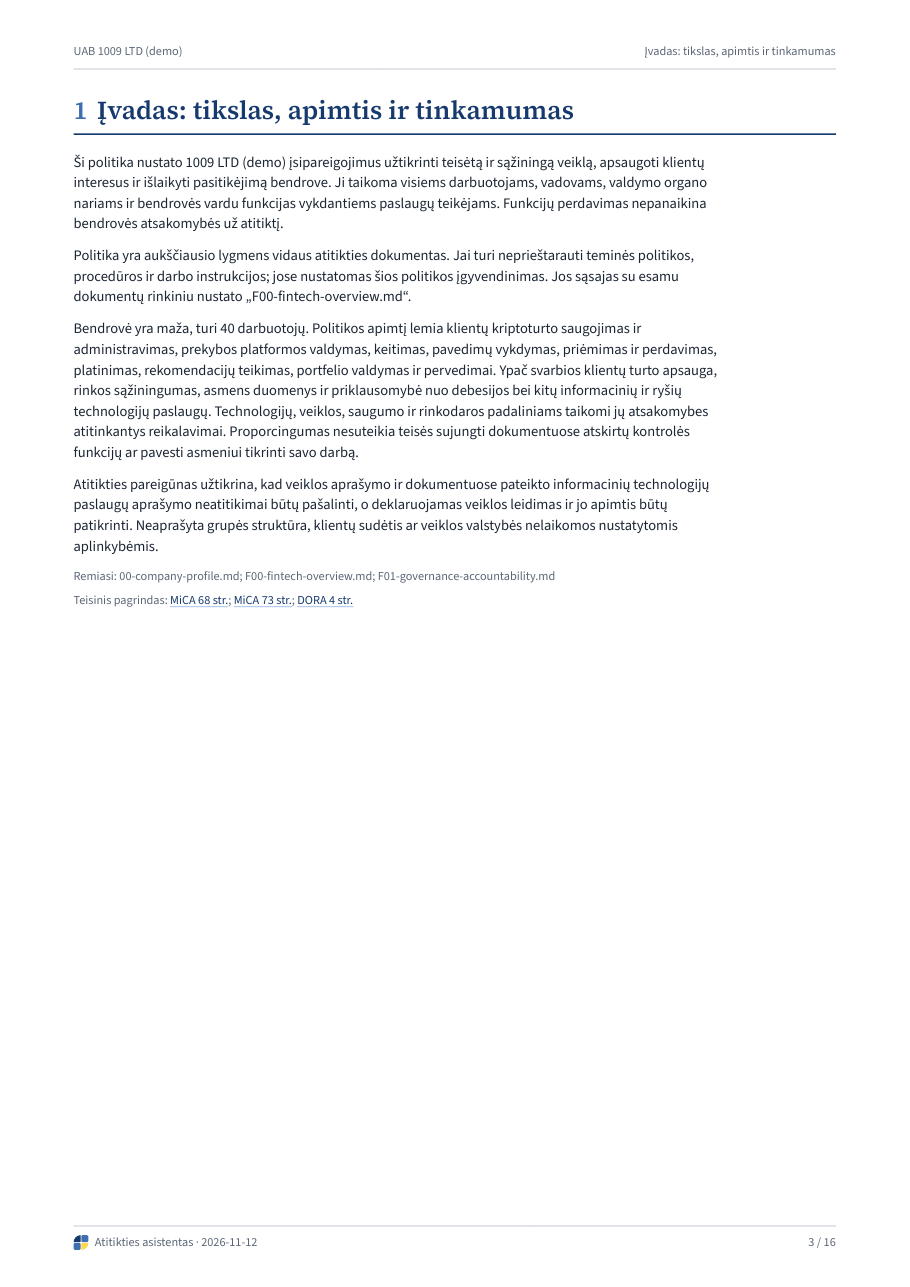
\includegraphics[width=.56\textwidth]{figures/samples/policy-part}
\caption{Sistemos PDF eksporto puslapis su pavyzdinės įmonės atitikties politika lietuvių
kalba (3 puslapis iš 16; politika sugeneruota 2026 m. lapkričio 12~d. duomenų bazės kopijoje):
pirmoji dalis, \enquote{Įvadas: tikslas, apimtis ir tinkamumas}. Po tekstu užrašas
\enquote{Remiasi} įvardija rinkinio dokumentus, kuriais dalis remiasi, o
\enquote{Teisinis pagrindas} --- nuostatas, kiekvieną su nuoroda į jos
šaltinį.}\label{fig:programme:policypage}
\end{figure}

\subsection{Pirmasis iškvietimas: politikos tekstas}

Be bendro bloko iškvietimas gauna įmonės klasifikaciją finansų rinkoje
(pateikiamą JSON formatu, kaip ir ataskaitos profilio tekste; \code{_context} faile
\file{programme/policy.py}), iki šešių įmonės turimų
rolių profilių (kiekvieną sutrumpintą iki 1\,200 ženklų), ataskaitos santrauką ir dalių sąrašą.
Instrukcija \prompt{programme.policy} prašo kiekvienai daliai 90--220 žodžių, kiekvienai
daliai --- vienos--trijų įmonės dokumentų ištraukų, cituojamų pažodžiui su dokumento nuoroda, ir
nuostatų, kurios dalies reikalauja ar ją pagrindžia. Instrukcijos griežtumą lemia dvi jos
ištraukos. Pirmoji pasako, kokio teksto norima:

\begin{promptexcerpt}{programme.policy}{kas yra politika ir kas ne}
WHAT A COMPLIANCE POLICY IS
It is the organisation's first-level document – its compliance "constitution". It says WHY the organisation complies and WHAT it commits to: principles, the compliance function's place and powers, who answers for what, which processes exist. It does not say HOW: procedures, forms, thresholds and step-by-step rules belong to the thematic policies and procedures below it, which the policy names where they exist. A policy that reads like a procedure, or like a copy of a standard, is a failed draft.
\end{promptexcerpt}

Antroji kalba apie tai, ko dokumentai neišsprendžia. Politika turi pasakyti, kam atsiskaito
atitikties pareigūnas ir kas gali jį atleisti, o dokumentų rinkinys to dažnai nepasako.
Modeliui liepiama sprendimą palikti atvirą, aiškiai tai parodant, ir įtraukti jį į sąrašą:

\begin{promptexcerpt}{programme.policy}{atviri klausimai pažymimi, niekada neužpildomi}
NEVER INVENT
Where the documents do not settle something the policy must state – to whom the compliance officer reports, who appoints and removes them, the review period, the budget rule – write the sentence with the open point in square brackets, in {LANGUAGE}, the way a drafter leaves a blank for the decision-maker (in Lithuanian "[Valdyba nusprendžia: …]"; in English "[The board to decide: …]"), and list each such point under `decisions`. Never put a name, a date, a number or an existing practice into the policy that the input does not give.
\end{promptexcerpt}

Puslapis ir PDF šiuos klausimus rodo po kiekviena dalimi kaip \ui{Sprendžia valdymo organas}, o
Word eksportas juos surenka pabaigoje. Dėl teisinio pagrindo instrukcija prašo teisės aktą
nurodyti tuo trumpuoju pavadinimu, kurį naudoja ataskaita, o straipsnį ir dalį --- vien
skaičiais (tokios formos reikia paieškai), ir baigiasi sakiniu, kuris instrukciją sieja su ją
lydinčia patikra:

\begin{promptexcerpt}{programme.policy}{teisinis pagrindas bus patikrintas}
[…]
Cite a provision only when you are sure the article is about that; three sure provisions are worth more than ten likely ones – every one will be checked against the official text. Standards (ISO 37301) and guidelines may be mentioned in the text, not in legalBasis.
\end{promptexcerpt}

\begin{pathcard}{Atitikties politika}{programme.policy}
  \pcrow{Trigger}{Užduoties \code{programme.generate} etapas \code{policy}, kai rengiamas
    \code{policy} rūšies dokumentas. Jį sukėlė naudotojas įmonės skiltyje \enquote{Programa}
    arba pokalbio įrankis \code{startWorkProduct}.}
  \pcrow{Input}{Bendras blokas: glaustas profilis ir visi dokumentai ištisai, daugiausia
    \code{DOCUMENT_PACK_CHARS}~=~600\,000 ženklų, kitaip generavimas sustoja. Duomenys:
    klasifikacija finansų rinkoje JSON formatu; pirmieji šeši rolių profiliai, po 1\,200 ženklų; ataskaitos
    santrauka su keturiais išvadų pavyzdžiais kiekvienai temai; aštuonios dalys, kurias reikia
    parašyti. Vienas iškvietimas, be paketų.}
  \pcrow{Prompt and model}{\prompt{programme.policy}, 1~versija, modelis \model{gpt-6.1-sol},
    temperatūra~0,2. Schema \code{POLICY_SCHEMA}, pavadinimu \code{policy}. Kintamieji
    \code{LANGUAGE}, \code{TODAY}, \code{COMPANY_NAME}. \enquote{Kantrus} iškvietimas: jis
    palaukia, kol praeis užklausų dažnio riba (\cref{ch:models}).}
  \pcrow{Output}{\code{title}; \code{parts[]}, kiekviena su \code{key} (viena iš aštuonių),
    \code{text}, \code{decisions[]}, \code{sources[]} iš \code{documentRef} ir \code{quote}
    bei \code{legalBasis[]} iš \code{act}, \code{article}, \code{paragraph}, \code{why}.}
  \pcrow{Checked by code}{\code{policy.validate}: dalys išdėstomos nustatyta tvarka su
    nustatytomis antraštėmis; kiekvienas tekstas sutrumpinamas iki 12\,000 ženklų ir turi
    turėti bent 150; kiekviena citata ieškoma savo dokumente; kiekviena nuostata ieškoma
    teisės aktų bazėje ir vieną kartą įvertinama (\cref{tab:programme:policyrules}).}
  \pcrow{Stored}{\code{work_products.content} (\code{title}, \code{parts}) su
    \code{checks}, \code{basis} ir \code{stats}. API podėlyje nieko nelaiko; bendrą bloką
    podėlyje laiko tiekėjas.}
  \pcrow{On failure}{Užduotis nekartojama. Dokumentas tampa \code{failed} su klaidos tekstu;
    ankstesnės versijos nepaliečiamos. Atšaukimo paisoma prieš prasidedant iškvietimui.}
  \pcrow{Cost}{Įskaitoma į generavimą pradėjusio naudotojo dienos biudžetą. Išmatuota
    2026 m. lapkričio 12~d. su \demo{} duomenimis: 0,46~\$ už visą politikos dokumentą, abu iškvietimus.}
  \pcrow{Human control}{Žmogus dokumento puslapyje redaguoja kiekvienos dalies tekstą,
    sprendimus ir teisinį pagrindą ir dokumentą patvirtina. Nepatvirtintas jis lieka
    projektas ir eksportuojamas kaip projektas.}
  \pcrow{Measured by}{Pačios instrukcijos niekas nematuoja. \file{tests/test_programme.py}
    su modelio imitacija testuoja aplink ją esantį kodą.}
\end{pathcard}

\subsection{Antrasis iškvietimas: hierarchija ir trūkstami dokumentai}

Antrasis iškvietimas prie to paties konteksto prideda rinkinio sąrašą --- kiekvieno dokumento
nuorodą, pavadinimą, tipą, kurį jam suteikė inventorius, ir pirmuosius 300 jo santraukos
ženklų --- ir ką tik parengtą politiką, kiekvieną dalį pagal raktą su pirmaisiais 500 jos
ženklų. Instrukcija \prompt{programme.documents} užduoda du klausimus. Pirmasis --- kurioje
vietoje yra kiekvienas esamas dokumentas:

\begin{promptexcerpt}{programme.documents}{dokumentų hierarchijos lygmenys}
THE THREE LEVELS
- 1 – the compliance policy and the code of ethics or conduct: WHY the organisation complies; approved by the governing body.
- 2 – thematic policies and standards: WHAT must be achieved in one field (prevention of money laundering, personal data, ICT security and resilience, conflicts of interest, safeguarding of client assets, outsourcing, complaints …).
- 3 – procedures, work instructions, plans, registers and forms: HOW it is done day to day, owned by the units that do the work.
- 0 – a text that is not a rule at all (a company profile, an overview, a report).
Go by what a document does, not by what its title calls it: a "policy" that sets out steps, forms and deadlines is level 3; a "procedure" that only states principles is level 2.
\end{promptexcerpt}

Antrasis --- kurių dokumentų trūksta. Modelis, paprašytas išvardyti trūkstamus dokumentus,
jų išvardys daug, todėl instrukcija šį žodį apibrėžia:

\begin{promptexcerpt}{programme.documents}{kada dokumentas laikomas trūkstamu}
[…]
A document is missing when all three hold:
1. something requires it – a provision of an act that binds the company (the acts of its report), or a process the drafted policy relies on (a compliance risk assessment method, a monitoring programme, reporting to the management, the breach-reporting channel, the disciplinary procedure, training);
2. no document of the library is dedicated to it; and
3. the gap changes what the company does: its staff would not know what to do, or the company could not show a supervisor how it does it.
[…]
\end{promptexcerpt}

Kiekvienas trūkstamas dokumentas pateikiamas su lygmeniu (2 arba 3), pavadinimu, paskirtimi,
politikos dalimi, kurią jis padaro įgyvendinamą (puslapyje ir PDF po paskirtimi nurodoma tos
dalies antraštė, o redaguojant projektą dalis parenkama iš pačios politikos dalių), prioritetu (\code{high}, \code{medium} ar
\code{low} --- instrukcija prašo panaudoti visus tris), jo reikalaujančia nuostata ir esamais
dokumentais, kurie tą dalyką jau iš dalies apima. Instrukcija liepia modeliui ataskaitos temą,
kurioje daug pareigų turi būseną \status{unknown}, laikyti ženklu, kad trūksta dokumento, ir
sąraše nurodyti dokumentą, o ne pareigą.

\begin{pathcard}{Dokumentų hierarchija ir trūkstami dokumentai}{programme.documents}
  \pcrow{Trigger}{To pačios užduoties etapas \code{document_gaps}, iškart po etapo
    \code{policy}.}
  \pcrow{Input}{Tas pats bendras blokas, žodis žodin. Duomenys: pirmojo iškvietimo
    klasifikacija, rolių profiliai ir ataskaitos santrauka; \enquote{THE LIBRARY}, po eilutę
    kiekvienam dokumentui (nuoroda, pavadinimas, inventoriaus nurodytas tipas arba deklaruota
    rūšis, 300 santraukos ženklų); \enquote{THE POLICY JUST DRAFTED}, kiekviena dalis pagal
    raktą su pirmaisiais 500 ženklų, kaip juos parašė pirmasis iškvietimas.}
  \pcrow{Prompt and model}{\prompt{programme.documents}, 1~versija, modelis
    \model{gpt-6.1-sol}, temperatūra~0,2. Schema \code{DOCUMENTS_SCHEMA}, pavadinimu
    \code{documents}. Tie patys trys kintamieji; \enquote{kantrus} iškvietimas.}
  \pcrow{Output}{\code{hierarchy[]}: \code{documentRef}, \code{level} (0, 1, 2, 3),
    \code{topic}, \code{note}. \code{missing[]}: \code{level} (2, 3), \code{title},
    \code{purpose}, \code{supports} (dalies raktas), \code{priority} (\code{high},
    \code{medium}, \code{low}), \code{legalBasis[]}, \code{partlyCoveredBy[]} (nuorodos).}
  \pcrow{Checked by code}{Nuorodos paverčiamos dokumentais. Hierarchijos eilutė, nurodanti
    nežinomą ar pasikartojantį dokumentą arba lygmenį už 0--3 ribų, atmetama; įspėjimas
    \code{hierarchy} įvardija dokumentus, likusius be lygmens (pirmuosius dvylika). Trūkstamas
    dokumentas be pavadinimo atmetamas; netinkamas lygmuo tampa 3, netinkama dalis ---
    \code{processes}, netinkamas prioritetas --- \code{medium}. Jo nuostatos pereina tą pačią
    paiešką ir tas pačias tris taisykles kaip ir dalių nuostatos.}
  \pcrow{Stored}{\code{work_products.content} (\code{hierarchy}, \code{missing}).}
  \pcrow{On failure}{Kaip ir pirmojo iškvietimo atveju; pirmojo iškvietimo atsakymas prarandamas kartu
    su generavimu, nes turinys išsaugomas tik pabaigoje.}
  \pcrow{Cost}{Generavimą pradėjęs naudotojas; tai dalis 0,46~\$, išmatuotų už dokumentą.}
  \pcrow{Human control}{Žmogus keičia bet kurio dokumento lygmenį ir temą, redaguoja ar
    pašalina trūkstamą dokumentą ir patvirtina dokumentą kaip visumą.}
  \pcrow{Measured by}{Pačios instrukcijos niekas nematuoja.}
\end{pathcard}

\subsection{Politikos taisyklės}

\begin{xltabular}{\textwidth}{@{}L{37mm}L{17mm}Y@{}}
\caption{Taisyklės, kurias tikrina \code{policy.validate}, ta tvarka, kuria ji jas pateikia}\label{tab:programme:policyrules}\\
\toprule
\hd{Taisyklė} & \hd{Pobūdis} & \hd{Laikomasi, kai} \\
\midrule
\endfirsthead
\toprule
\hd{Taisyklė} & \hd{Pobūdis} & \hd{Laikomasi, kai} \\
\midrule
\endhead
\bottomrule
\endlastfoot
\code{parts} & privaloma & Kiekviena iš aštuonių dalių turi bent \code{MIN_PART_CHARS}~=~150 teksto ženklų. Dalis, kurios turinyje nėra, laikoma tuščia. \\
\code{provisions} & privaloma & Nė viena dalies ar trūkstamo dokumento nurodyta nuostata neturi būsenos \code{not_found}. \\
\code{provisions_unverified} & įspėjimas & Nė viena nuostata nenurodo teisės akto, kurio bazėje nėra. \\
\code{provision_subjects} & įspėjimas & Nė viena nuostata nebuvo įvertinta kaip \code{mismatch}. \\
\code{quotes} & įspėjimas & Kiekviena kiekvienos dalies citata yra dokumente, kurį ji nurodo. \\
\code{hierarchy} & įspėjimas & Kiekvienas įmonės dokumentas turi lygmenį. Po generavimo įkeltas dokumentas jo neturi. \\
\end{xltabular}

Taisyklės parodo, kad politika išsami ir kad jos nuorodos egzistuoja. Jos neparodo, kad tai
gera politika: ar mandatas pakankamai stiprus, ar trūkstamo dokumento tikrai trūksta, ar
lygmuo parinktas teisingai --- sprendžia žmogus, skaitantis projektą.


% ------------------------------------------------------------
\section{Valdymo struktūra, atitikties procesas ir RACI}\label{sec:programme:governance}

Valdymo struktūros dokumentas (\file{programme/governance.py}) parodo, kas atsakingas už
atitiktį. Pirmasis jo iškvietimas iš rinkinio nustato, kokia organizacija yra, ir pasiūlo,
kokia ji turėtų būti; antrasis suprojektuoja atitikties valdymo procesą ir paskirsto kiekvieną
jo etapą. Paties modulio komentaras nurodo šio darbo ribą: RACI matrica yra joje esančių žmonių
susitarimas, o tai, kas gaunama čia, --- projektas, nuo kurio jie pradeda.

\subsection{Pirmasis iškvietimas: pareigybės, spragos ir struktūra}

Be bendro bloko iškvietimas gauna roles, kurias išvardija kiekvieno dokumento inventorius (su
nurodymu jas patikrinti dokumentuose), tris politikos dalis, įvardytas
\cref{sec:programme:what}, ir ataskaitos santrauką. Instrukcija \prompt{programme.structure}
prašo trijų sąrašų. \code{positions} --- tai pareigybės, organai ir padaliniai, kuriuos
dokumentai iš tikrųjų įvardija, kiekviena su savo padaliniu, \term{linija} (\code{governing},
\code{first}, \code{second}, \code{third} arba \code{external}, pagal trijų linijų modelį),
vienu pareigas nusakančiu sakiniu ir viena ar dviem pažodžiui cituojamomis ištraukomis.
\code{gaps} --- tai rolės, kurių tokios rūšies ir dydžio finansų rinkos dalyviui reikia, o
dokumentai jų neparodo arba parodo taip, kad jos negali veikti; instrukcija pirmiausia
nukreipia dėmesį į antrosios linijos nepriklausomumą. \code{structure} --- tai siūloma
organizacija kaip mazgų medis: kiekvienas mazgas yra \code{body}, \code{committee},
\code{function} arba \code{unit} ir turi id, liniją, mazgo, kuriam jis pavaldus, id, pastabą ir
žymą \code{proposed}, kuri įjungiama tik tam mazgui, kurio dokumentai visai neįvardija.
Instrukcija nurodo taisykles, kurių medis turi laikytis:

\begin{promptexcerpt}{programme.structure}{medžio taisyklės}
[…]
   - the top is the governing body (the shareholders' meeting need not be drawn); a supervisory board, where the company has one, stands above the management board;
   - the first line hangs under the chief executive or the management board;
   - a second-line function reports to the management board or the chief executive and never to a first-line unit; show its direct access to the governing body in the note, not by a second parent – a node has one parent;
   - internal audit, the third line, reports to the supervisory board, or to the management board where there is no supervisory board – never to the chief executive's line;
   - keep it proportionate: for a firm of this size a handful of committees at most, and no node without a job. Fifteen to twenty-five nodes are usually enough.
\end{promptexcerpt}

\begin{pathcard}{Pareigybės ir valdymo struktūra}{programme.structure}
  \pcrow{Trigger}{Užduoties \code{programme.generate} etapas \code{structure}, kai rengiamas
    \code{governance} rūšies dokumentas.}
  \pcrow{Input}{Bendras blokas. Duomenys: \enquote{ROLES EACH DOCUMENT NAMES}, po eilutę
    kiekvienam dokumentui su jo inventoriaus \code{roles}; politikos dalys \code{mandate},
    \code{roles} ir \code{processes}, po 1\,800 ženklų, su politikos versija ir žinia, ar ji
    patvirtinta, --- arba pranešimas, kad politikos dokumento nėra; ataskaitos santrauka su
    dviem pavyzdžiais kiekvienai temai.}
  \pcrow{Prompt and model}{\prompt{programme.structure}, 1~versija, modelis
    \model{gpt-6.1-sol}, temperatūra~0,2. Schema \code{STRUCTURE_SCHEMA}, pavadinimu
    \code{structure}. \enquote{Kantrus} iškvietimas.}
  \pcrow{Output}{\code{title}; \code{positions[]}: \code{name}, \code{unit}, \code{line}
    (\code{governing}, \code{first}, \code{second}, \code{third}, \code{external}),
    \code{duties}, \code{sources[]}; \code{gaps[]}: \code{role}, \code{line}, \code{why};
    \code{structure[]}: \code{id}, \code{name}, \code{kind} (\code{body}, \code{committee},
    \code{function}, \code{unit}), \code{line}, \code{parentId}, \code{proposed}, \code{note}.}
  \pcrow{Checked by code}{\code{governance.validate}: citatos ieškomos dokumentuose
    (įspėjimas \code{quotes}); mazgas be pavadinimo ar su pasikartojančiu id atmetamas;
    tėvinis mazgas, kuris nėra mazgas arba kuris uždarytų ratą, atkerpamas; privalomos
    taisyklės \code{structure} ir \code{independence} (\cref{tab:programme:govrules}).}
  \pcrow{Stored}{\code{work_products.content} (\code{title}, \code{positions}, \code{gaps},
    \code{structure}).}
  \pcrow{On failure}{Nekartojama; dokumentas tampa \code{failed}.}
  \pcrow{Cost}{Generavimą pradėjęs naudotojas. Išmatuota 2026 m. lapkričio 12~d. su \demo{} duomenimis:
    0,39~\$ už visą valdymo struktūros dokumentą, abu iškvietimus.}
  \pcrow{Human control}{Žmogus redaguoja, prideda ir šalina struktūros mazgus ir patvirtina
    dokumentą kaip visumą; pareigybės ir spragos puslapyje neredaguojamos --- kaip įrašas apie
    tai, kas rasta.}
  \pcrow{Measured by}{Pačios instrukcijos niekas nematuoja.}
\end{pathcard}

\subsection{Antrasis iškvietimas: procesas ir matrica}

Antrasis iškvietimas gauna siūlomos struktūros mazgus --- id, pavadinimą, liniją ir ar mazgas
siūlomas --- po antrašte \enquote{ROLES OF THE STRUCTURE (use these ids)}, taip pat tas pačias
politikos dalis ir ataskaitos santrauką. Instrukcija \prompt{programme.raci} prašo vieno
proceso iš aštuonių--keturiolikos etapų, išdėstytų metų darbo tvarka, kiekvieną pavadintą jo
atliekamu veiksmu, su aprašymu, periodiškumu ir pagrindu: ISO~37301:2021 punktu arba Lietuvos
banko gairių dėl atitikties funkcijos (2022) punktu, kurį etapas įgyvendina. Instrukcija
išvardija punktus, kuriuos modelis gali naudoti, ir apie ką kiekvienas iš jų, todėl modelis
renkasi iš sąrašo. Tada eina matrica:

\begin{promptexcerpt}{programme.raci}{auksinė taisyklė ir kas už jos ribų}
THE MATRIX
raci – for every step, which roles take part: R (responsible – does the work), A (accountable – answers for the result and signs it off), AR (both), C (consulted – asked before, two-way), I (informed – told after, one-way). One entry per step and role that takes part; a role with no part in a step gets no entry.
The golden rule, which will be checked: every step has EXACTLY ONE accountable role and AT LEAST ONE responsible role. A role holds one value in a step: R, A, C, I – or AR where the role that does the work also answers for its result. Prefer to separate the two (the one who answers checks the one who does); use AR where the company is too small for that in the step.
Beyond the rule:
- The first line owns its risks: where a step is done in the business (applying controls, correcting a finding), the business unit is R and its manager or the chief executive A; compliance is C or monitors – the second line does not repair what it finds.
[…]
- Internal audit is never R or A in a step it will later audit; it is I, or R only for the independent review of the system.
[…]
\end{promptexcerpt}

\begin{pathcard}{Atitikties procesas ir RACI matrica}{programme.raci}
  \pcrow{Trigger}{To pačios užduoties etapas \code{process_raci}, iškart po etapo
    \code{structure}.}
  \pcrow{Input}{Tas pats bendras blokas. Duomenys: kiekvienas pirmojo iškvietimo pasiūlytas
    mazgas, po eilutę mazgui su jo id, pavadinimu ir linija, o kur taikoma --- su žodžiu
    \enquote{proposed}; tos pačios politikos dalys ir ataskaitos santrauka.}
  \pcrow{Prompt and model}{\prompt{programme.raci}, 1~versija, modelis \model{gpt-6.1-sol},
    temperatūra~0,2. Schema \code{RACI_SCHEMA}, pavadinimu \code{raci}. \enquote{Kantrus}
    iškvietimas.}
  \pcrow{Output}{\code{steps[]}: \code{id}, \code{name}, \code{description},
    \code{frequency}, \code{basis[]} iš \code{source} (\code{ISO 37301} arba \code{LB gairės})
    ir \code{ref}. \code{raci[]}: \code{stepId}, \code{roleId}, \code{value} (\code{R},
    \code{A}, \code{AR}, \code{C}, \code{I}).}
  \pcrow{Checked by code}{Etapas be id ar pavadinimo arba su pasikartojančiu id atmetamas.
    Langelis, nenurodantis jokio etapo, jokio struktūros mazgo ar tinkamos raidės, atmetamas;
    jei vienai rolei viename etape nurodytos kelios raidės, galioja paskutinė. Privalomos
    taisyklės \code{process}, \code{raci_accountable}, \code{raci_responsible}; įspėjimai
    \code{raci_everywhere}, \code{raci_heavy}, \code{process_basis}.}
  \pcrow{Stored}{\code{work_products.content} (\code{process}, \code{raci}).}
  \pcrow{On failure}{Nekartojama; pirmojo iškvietimo atsakymas prarandamas kartu su
    generavimu.}
  \pcrow{Cost}{Generavimą pradėjęs naudotojas; tai dalis 0,39~\$, išmatuotų už dokumentą.}
  \pcrow{Human control}{Žmogus redaguoja etapus ir kiekvieną matricos langelį. Puslapis
    pažymi auksinę taisyklę pažeidžiantį etapą, vos tik pasikeičia langelis; ar dokumentą
    galima patvirtinti, sprendžia serverio patikra išsaugant.}
  \pcrow{Measured by}{Pačios instrukcijos niekas nematuoja.}
\end{pathcard}

\begin{figure}[H]
\centering
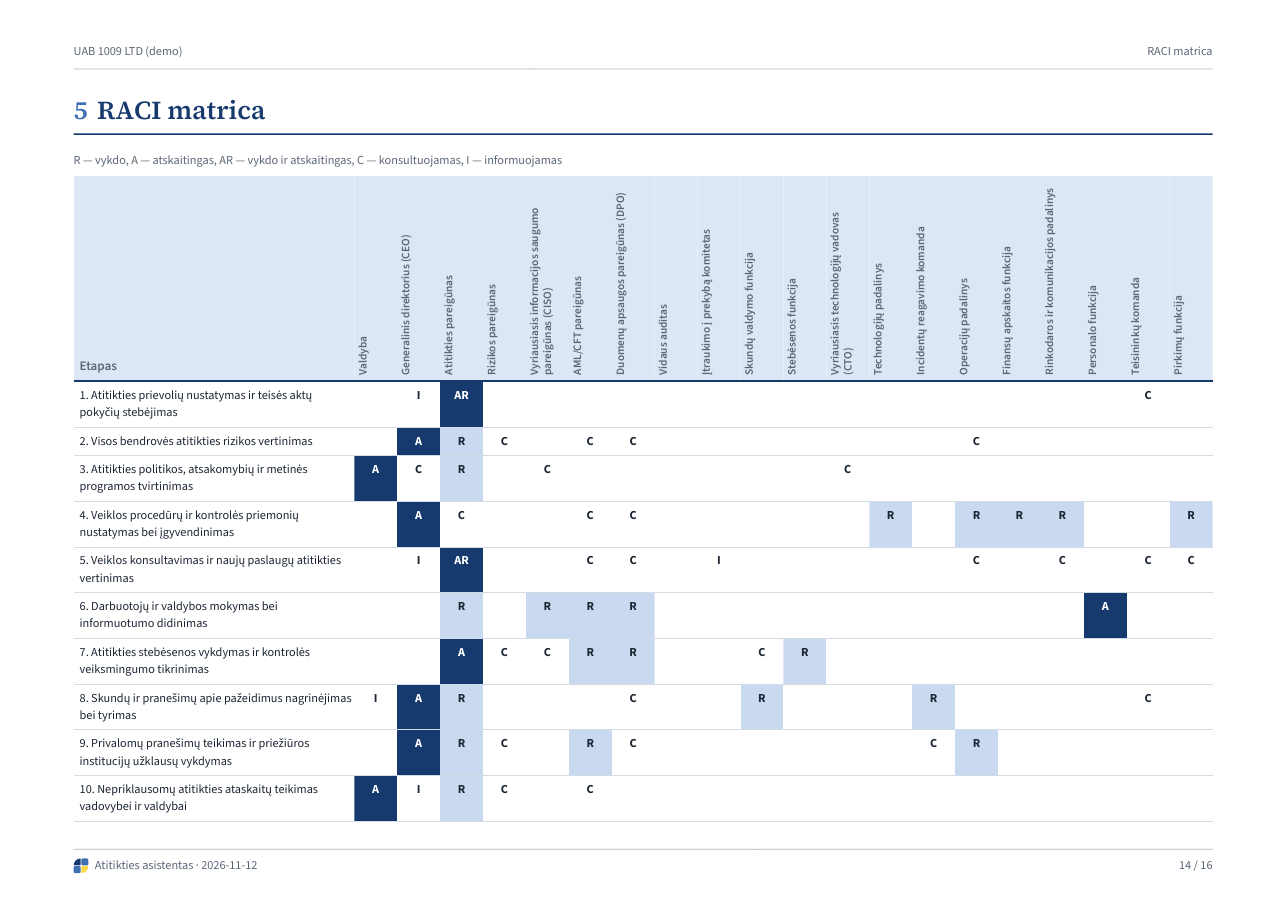
\includegraphics[width=\textwidth]{figures/samples/governance-raci}
\caption{RACI matrica, kaip ją pavyzdinei įmonei lietuvių kalba spausdina sistemos PDF
eksportas (14 puslapis iš 16; valdymo struktūros dokumentas sugeneruotas 2026 m. lapkričio
12~d. duomenų bazės kopijoje; gulsčias puslapis). Po eilutę kiekvienam proceso etapui, po
stulpelį kiekvienai struktūros rolei; A ir AR --- tamsiai mėlyname fone, R --- šviesiai
mėlyname, C ir I --- paprastos raidės. Puslapyje telpa pirmieji dešimt iš keturiolikos etapų,
kiekvienas su lygiai viena A arba AR.}\label{fig:programme:racipage}
\end{figure}

\subsection{Valdymo struktūros dokumento taisyklės}

Dvi taisyklių grupės yra struktūrinės ir privalomos: medis su jo gynybos linijomis ir matricos
auksinė taisyklė. Abi suskaičiuoja kelios \code{governance.validate} eilutės.

\begin{codebox}{Gynybos linijos ir auksinė taisyklė, kaip jas užrašo kodas}
Antrosios linijos mazgas negali būti pavaldus pirmosios linijos mazgui. Trečiosios linijos
mazgas, turintis tėvinį mazgą, gali būti pavaldus tik valdymo linijos mazgui. Bet kuri kita
vieta šiai taisyklei tinka; antrosios ar trečiosios linijos mazgą be tėvinio mazgo vietoj jos
sugauna taisyklė \code{structure}:

\begin{codeblock}
subordinated = [node["name"] for node in nodes if node["line"] == "second" and node["parentId"]
                and by_id[node["parentId"]]["line"] == "first"]
subordinated += [node["name"] for node in nodes if node["line"] == "third" and node["parentId"]
                 and by_id[node["parentId"]]["line"] != "governing"]
\end{codeblock}

Matricai \code{cells} susieja etapą ir rolę su viena reikšme. Raidė skaičiuojama visur, kur ji
yra reikšmėje, todėl \code{AR} skaičiuojama vieną kartą kaip atskaitinga ir vieną kartą kaip
vykdanti rolė:

\begin{codeblock}
letters = lambda step_id, letter: sum(letter in value for (cell_step, _), value in cells.items() if cell_step == step_id)
accountable = [step["name"] for step in steps if letters(step["id"], "A") != 1]
responsible = [step["name"] for step in steps if letters(step["id"], "R") < 1]
\end{codeblock}

Etapas įrašomas į \code{raci_accountable}, kai neturi nė vienos atskaitingos rolės arba turi
daugiau nei vieną, ir į \code{raci_responsible}, kai darbo niekas neatlieka. Procesas be etapų
pažeidžia abi taisykles.
\end{codebox}

\begin{xltabular}{\textwidth}{@{}L{34mm}L{17mm}Y@{}}
\caption{Taisyklės, kurias tikrina \code{governance.validate}, ta tvarka, kuria ji jas pateikia}\label{tab:programme:govrules}\\
\toprule
\hd{Taisyklė} & \hd{Pobūdis} & \hd{Laikomasi, kai} \\
\midrule
\endfirsthead
\toprule
\hd{Taisyklė} & \hd{Pobūdis} & \hd{Laikomasi, kai} \\
\midrule
\endhead
\bottomrule
\endlastfoot
\code{structure} & privaloma & Struktūra turi bent vieną mazgą; kiekvienas mazgas be tėvinio mazgo yra valdymo arba išorės linijoje, ir bent vienas iš jų --- valdymo linijoje; ir joks mazgas nenurodo tėvinio mazgo, kuris nėra mazgas. \\
\code{independence} & privaloma & Joks antrosios linijos mazgas nėra pavaldus pirmosios linijos mazgui ir joks trečiosios linijos mazgas nėra pavaldus mazgui, kuris nepriklauso valdymo linijai. \\
\code{process} & privaloma & Procesą sudaro bent \code{MIN_STEPS}~=~5 etapai. \\
\code{raci_accountable} & privaloma & Etapų yra, ir kiekvienas etapas turi lygiai vieną rolę, kurios reikšmėje yra A. \\
\code{raci_responsible} & privaloma & Etapų yra, ir kiekvienas etapas turi bent vieną rolę, kurios reikšmėje yra R. \\
\code{raci_everywhere} & įspėjimas & Nė viena rolė neturi raidės kiekviename etape. \\
\code{raci_heavy} & įspėjimas & Nė viena rolė nėra atskaitinga daugiau nei pusėje etapų. \\
\code{process_basis} & įspėjimas & Kiekvienas etapas turi bent vieną pagrindo įrašą, nurodantį žinomą punktą. \\
\code{quotes} & įspėjimas & Kiekviena kiekvienos pareigybės citata yra dokumente, kurį ji nurodo. \\
\end{xltabular}

Prieš tikrinant taisykles struktūra pačia konstrukcija paverčiama mišku: mazgas, kurio tėvinis
mazgas nėra mazgas, yra jis pats arba uždarytų ratą, netenka tėvinio mazgo ir tampa viršutiniu mazgu.
Taisyklė \code{structure} tada reikalauja, kad kuris nors viršutinis mazgas būtų valdymo organas
ir kad niekas kitas nekabėtų ore: viršuje stovi valdymo organas, išorės subjektas ---
auditorius, priežiūros institucija --- gali stovėti šalia medžio, o kiekvienas kitas mazgas turi
savo vietą po kuriuo nors mazgu. Mazgas, nurodęs tėvinį mazgą, kuris nėra mazgas, ir viršutinis
mazgas bet kurioje linijoje, išskyrus valdymo ir išorės linijas, pavadinimais išvardijami
taisyklės detalėse (\code{detached} funkcijoje \code{governance.validate}), kad padalinys, kurį
modelis paliko niekur nepriskirtą, būtų pastebėtas dar prieš patvirtinant struktūros schemą,
kurioje jis būtų nubraižytas kaip antra organizacijos viršūnė.
\code{process_basis} atveju kodas žino, kurios nuorodos egzistuoja: aibėje \code{ISO_CLAUSES}
yra 41 ISO~37301:2021 punkto numeris nuo 4.1 iki 10.2, o gairių punktas laikomas žinomu, kai jo
numeris yra nuo 1 iki 79 (\code{GUIDELINE_PARAGRAPHS}). Nuoroda už abiejų ribų turinyje
paliekama; etapas, kurio nė viena nuoroda nežinoma, įvardijamas įspėjimo detalėse.

Du matricos įspėjimai pakartoja tai, ką instrukcija sako žodžiais: rolė, turinti raidę
kiekviename etape, daro per daug arba įrašyta iš įpratimo, o rolė, atskaitinga už daugumą
etapų, tampa siaurąja vieta. Tai įspėjimai, nes mažoje įmonėje kitos išeities gali nebūti; sprendžia
peržiūrėtojas.


% ------------------------------------------------------------
\section{Teisinė rizika: kriterijai, scenarijai ir registras}\label{sec:programme:risks}

Rizikos dokumentas (\file{programme/risks.py}) laikosi ISO~31022 teisinės rizikos valdymo
metodo, kaip jį dėsto kursas: pirmiausia kriterijai, paskui pagal juos 5×5 matricoje vertinami
scenarijai. Darbas pasidalytas griežtai. Modelis formuluoja kriterijus, rašo scenarijus ir
vertina juos pagal aštuonis aspektus. Kodui priklauso viskas, kas yra skaičius ar nustatyta
skalė: lygių pavadinimai, rizikos lygiai ir kiekvieno iš jų leidžiami reagavimo būdai,
tikimybė, poveikis, balas, rizikos lygis ir id.

\subsection{Kriterijai ir rizikos lygiai}

Kriterijai --- tai dvi lentelės: penki lygiai pagal keturis aspektus
(\cref{tab:programme:criteria}). Lygių pavadinimai ir aspektų raktai yra konstantos; modelis
užpildo keturiasdešimt langelių, kiekviename --- šešių--dvidešimties žodžių frazę, pagal kurią
lygį galima atpažinti.

\begin{table}[H]
\caption{Dvi kriterijų pusės (\code{LIKELIHOOD}, \code{IMPACT} ir jų aspektai)}\label{tab:programme:criteria}
\begin{tabularx}{\textwidth}{@{}L{20mm}L{48mm}Y@{}}
\toprule
\hd{Pusė} & \hd{1--5 lygiai} & \hd{Aspektai} \\
\midrule
Tikimybė & Labai mažai tikėtina, Mažai tikėtina, Vidutiniškai tikėtina, Tikėtina, Beveik neabejotina &
  \code{control} --- vidaus kontrolė ir kompetencija; \code{clarity} --- teisinis aiškumas ir
  priežiūros praktika; \code{counterparty} --- kontrahentų ir trečiųjų šalių patikimumas;
  \code{frequency} --- dažnumas ir tikimybė laike \\
Poveikis & Nereikšmingas, Mažas, Vidutinis, Didelis, Katastrofinis &
  \code{financial} --- finansinis poveikis; \code{regulatory} --- teisinis, priežiūrinis ir
  licencinis poveikis; \code{reputation} --- reputacija ir nematerialusis turtas;
  \code{reach} --- skvarba, mastas ir domino efektas \\
\bottomrule
\end{tabularx}
\end{table}

Instrukcija \prompt{programme.risk_criteria} kiekvienam aspektui pateikia atramą ---
\code{frequency}, \code{regulatory}, \code{reputation} ir \code{reach} atveju formuluotę
kiekvienam iš penkių lygių --- ir prasideda testu, kurį kriterijai turi išlaikyti:

\begin{promptexcerpt}{programme.risk_criteria}{kada kriterijais galima naudotis}
[…]
The criteria will be used to score risk scenarios on a 5×5 matrix (likelihood × impact), and the governing body approves them: they must be concrete enough that two people scoring the same risk arrive at the same level.
\end{promptexcerpt}

Būtent pinigų srityje bendriniai kriterijai mažai įmonei netinka, todėl finansiniam aspektui
liepiama prisitaikyti prie įmonės mastelio ir nurodyti, kokias prielaidas jis padarė:

\begin{promptexcerpt}{programme.risk_criteria}{finansinė skalė}
- financial – the direct loss, fine or cost. Scale it to THIS company, not to a bank: give each level as a share of the company's annual income (or of its own funds) and, only when the profile states the turnover, also in euros. When the turnover is not stated, give the shares, add a euro range a company of this size and licence class would plausibly use, mark it as an assumption in `calibration`, and say it must be replaced once the figure is known.
\end{promptexcerpt}

Tas pats iškvietimas parašo \term{rizikos apetitą}: kiekvienam iš penkių rizikos lygių --- ką
tokio lygio rizika reiškia šiai įmonei ir kas dėl jos sprendžia. Pačių rizikos lygių modelio
neprašoma. Konstanta \code{BANDS} saugo jų balų intervalus, pavadinimus ir kiekvieno leidžiamus
reagavimo būdus; iškvietimui jie parodomi po antrašte
\enquote{THE BANDS OF THE MATRIX (fixed)}, o \code{validate} apetitą atkuria lygį po lygio iš
konstantos ir iš atsakymo paima tik du tekstus.

\begin{table}[H]
\caption{Matricos rizikos lygiai (\code{BANDS})}\label{tab:programme:bands}
\begin{tabularx}{\textwidth}{@{}L{24mm}L{16mm}L{44mm}Y@{}}
\toprule
\hd{Rizikos lygis} & \hd{Balas} & \hd{Pavadinimas} & \hd{Leidžiami reagavimo būdai} \\
\midrule
\code{negligible} & 1--3 & Nereikšminga & priimti, didinti \\
\code{tolerable} & 4--6 & Toleruotina & priimti, mažinti \\
\code{medium} & 8--12 & Vidutinė & mažinti, perkelti \\
\code{high} & 15--16 & Didelė & mažinti, vengti \\
\code{critical} & 20--25 & Kritinė & vengti \\
\bottomrule
\end{tabularx}
\end{table}

\begin{pathcard}{Teisinės rizikos kriterijai ir apetitas}{programme.risk_criteria}
  \pcrow{Trigger}{Užduoties \code{programme.generate} etapas \code{criteria}, kai rengiamas
    \code{risks} rūšies dokumentas.}
  \pcrow{Input}{Bendras blokas. Duomenys: įmonės mastas (dydžio kategorija, darbuotojų
    skaičius, metinė apyvarta eurais arba žymė \enquote{not stated}); penki rizikos lygiai su
    jų intervalais, pavadinimais ir leidžiamais reagavimo būdais iš \code{BANDS}; ataskaitos
    santrauka su vienu pavyzdžiu kiekvienai temai.}
  \pcrow{Prompt and model}{\prompt{programme.risk_criteria}, 1~versija, modelis
    \model{gpt-6.1-sol}, temperatūra~0,2. Schema \code{CRITERIA_SCHEMA}, pavadinimu
    \code{risk_criteria}. \enquote{Kantrus} iškvietimas.}
  \pcrow{Output}{\code{likelihood[]}: \code{level} (1--5), \code{control}, \code{clarity},
    \code{counterparty}, \code{frequency}. \code{impact[]}: \code{level}, \code{financial},
    \code{regulatory}, \code{reputation}, \code{reach}. \code{appetite[]}: \code{band}
    (\code{negligible}, \code{tolerable}, \code{medium}, \code{high}, \code{critical}),
    \code{comment}, \code{decision}. \code{calibration}.}
  \pcrow{Checked by code}{Abi lentelės atkuriamos 1--5 lygiams su kodo nustatytais lygių
    pavadinimais, kiekvienas langelis sutrumpinamas iki 500 ženklų. Apetitas atkuriamas iš
    \code{BANDS}: intervalas, pavadinimas ir reagavimo būdai yra kodo, tik \code{comment} ir
    \code{decision} --- modelio; sprendimas apribojamas iki 1\,000 ženklų, o kriterijų
    pritaikymo paaiškinimas --- iki 4\,000 (\code{DECISION_CHARS}, \code{CALIBRATION_CHARS}).
    Tuščias langelis, rizikos lygis be komentaro ar sprendimo arba trūkstamas kriterijų
    pritaikymo paaiškinimas pažeidžia privalomą taisyklę \code{criteria}.}
  \pcrow{Stored}{\code{work_products.content} (\code{criteria} su \code{likelihood},
    \code{impact} ir \code{calibration}; \code{appetite}).}
  \pcrow{On failure}{Nekartojama; dokumentas tampa \code{failed}.}
  \pcrow{Cost}{Generavimą pradėjęs naudotojas. Išmatuota 2026 m. lapkričio 12~d. su \demo{} duomenimis:
    nuo 0,35 iki 0,48~\$ už visą rizikos dokumentą, abu iškvietimus.}
  \pcrow{Human control}{Žmogus perrašo bet kurį langelį, pastabą apie kalibravimą ir kiekvieno
    rizikos lygio reikšmę bei sprendimą; rizikos lygių, jų intervalų ir reagavimo būdų
    redaguoti negalima.}
  \pcrow{Measured by}{Pačios instrukcijos niekas nematuoja.}
\end{pathcard}

\subsection{Scenarijai}

\term{Scenarijus} --- tai viena įmonės teisinė rizika, nusakyta vienu nustatytos formos
sakiniu ir apsupta to, ką apie ją įrašo registras. Antrasis iškvietimas gauna kriterijus,
kaip juos suformulavo pirmasis iškvietimas, keturias tipologijas, valdymo struktūros
padalinius (arba nurodymą naudoti dokumentuose įvardytus padalinius), rinkinį kaip nuorodas ir
pavadinimus ir rimčiausias atviras naujausios ataskaitos išvadas. Instrukcija
\prompt{programme.risk_scenarios} įtvirtina sakinio formą:

\begin{promptexcerpt}{programme.risk_scenarios}{sakinys, kurio laikosi kiekvienas scenarijus}
THE SENTENCE
Each scenario is ONE sentence of four parts, in this form:
- in Lithuanian: "Tikėtinas [rizikos įvykis], kylantis iš [rizikos šaltinio], gali sukelti [pasekmes], kurios paveiks [saugomą tikslą]." – adjust the endings so the sentence is correct ("Tikėtina", "kylanti", "pasekmę, kuri paveiks"), but keep the four parts in this order and the words that join them ("Tikėtin…", "kylan…", "gali sukelti", "paveiks");
- in English: "A likely [risk event], arising from [risk source], may cause [consequences] that will affect [protected objective]."
\end{promptexcerpt}

Keturios dalys --- įvykis, šaltinis, pasekmės, tikslas --- grąžinamos ir kaip keturi laukai,
kad kodas galėtų nustatyti, ar kurios nors trūksta. Kiekvienas scenarijus nurodo vieną ar dvi
iš šešių ISO~31022 A priedo teisinės rizikos rūšių (\cref{tab:programme:types}) ir po vieną
reikšmę iš kiekvienos iš dar trijų kode laikomų tipologijų: šešių šaltinių rūšių (nuo
reguliuotojų ir įstatymų leidėjų iki vidaus procesų ir IT), penkių pasekmių rūšių ir penkių
saugomų tikslų rūšių.
Tai paskaitos tipologijos, ir registras jas pateikia paskaitos žodžiais: po scenarijaus
teisinės rizikos rūšimis kortelėje, PDF ir darbaknygėje įvardijama jo šaltinio, pasekmių ir
saugomo tikslo rūšis (\enquote{Šaltinio rūšis},
\enquote{Pasekmių rūšis}, \enquote{Saugomo tikslo rūšis}; \code{TYPOLOGIES} faile
\file{programme/exports.py} ir konsolės faile \file{pages/Programme/programmeUtils.js}).

\begin{table}[H]
\caption{Teisinės rizikos rūšys (\code{CATEGORIES}) ir žodžiai, kuriais instrukcija kiekvieną paaiškina}\label{tab:programme:types}
\begin{tabularx}{\textwidth}{@{}rL{58mm}Y@{}}
\toprule
 & \hd{Rūšis} & \hd{Instrukcijos žodžiais} \\
\midrule
1 & Teisinės aplinkos nenuspėjamumas & teisė keičiasi arba yra neaiški \\
2 & Taikytinų teisės aktų nesilaikymas & įmonė nesilaiko ją saistančio teisės akto \\
3 & Sutarties pažeidimas & įmonė ar jos kontrahentas pažeidžia sutartį \\
4 & Trečiųjų asmenų teisių pažeidimas & įmonė pažeidžia kieno nors teises (klientų, duomenų subjektų, intelektinės nuosavybės teisių turėtojų) \\
5 & Neveikimas įgyvendinant teises & įmonė nepasinaudoja turima teise (reikalauti, nutraukti, priverstinai įgyvendinti, apsidrausti) \\
6 & Netinkamas pasirinkimas & įmonė teisiškai prastai pasirenka (struktūrą, kontrahentą, jurisdikciją, sutarties sąlygą) \\
\bottomrule
\end{tabularx}
\end{table}

Aplink sakinį modelis parašo veiklos sritį ir padalinį, kuriam rizika priklauso; vieno--trijų
rinkinio dokumentų, su kuriais susijęs scenarijus, nuorodas; teisinį pagrindą; \term{vidaus
išvadą} --- ką įmonės dokumentai ir naujausia ataskaita šiandien rodo apie šią riziką; lygį nuo
1 iki 5 pagal kiekvieną iš aštuonių aspektų su pagrindimu kiekvienai pusei; reagavimo būdą;
du--keturis veiksmus; vieną ar du atsakingus asmenis; ir terminą ketvirčio tikslumu.
Instrukcija prašo šešių--dešimties scenarijų, apimančių bent penkias iš šešių rūšių; toliau
aprašytos taisyklės reikalauja penkių scenarijų, apimančių keturias, --- tai sąmoningai palikta
atsarga. Dėl vertinimo instrukcija
aiškiai pasako, ko modelis daryti neturi:

\begin{promptexcerpt}{programme.risk_scenarios}{kaip vertinti ir ko neskaičiuoti}
[…]
Score the impact of the reasonably foreseeable serious case – what would follow if the event happened as the scenario describes and the supervisor or the injured party acted on it – neither the mildest outcome nor the theoretical maximum, and say in `why` which case you scored.
[…]
Score what the input shows, not what would make a tidy matrix: a risk whose control is documented and tested is low on control however grave its impact, and not every risk of a regulated firm is high. Do not compute a total: the register takes the likelihood as the rounded mean of its four levels, the impact as the highest of its four, and their product as the score.
\end{promptexcerpt}

\Cref{fig:programme:registerpage} rodo du tikro registro scenarijus su viskuo, kas yra aplink
sakinį.

\begin{figure}[H]
\centering
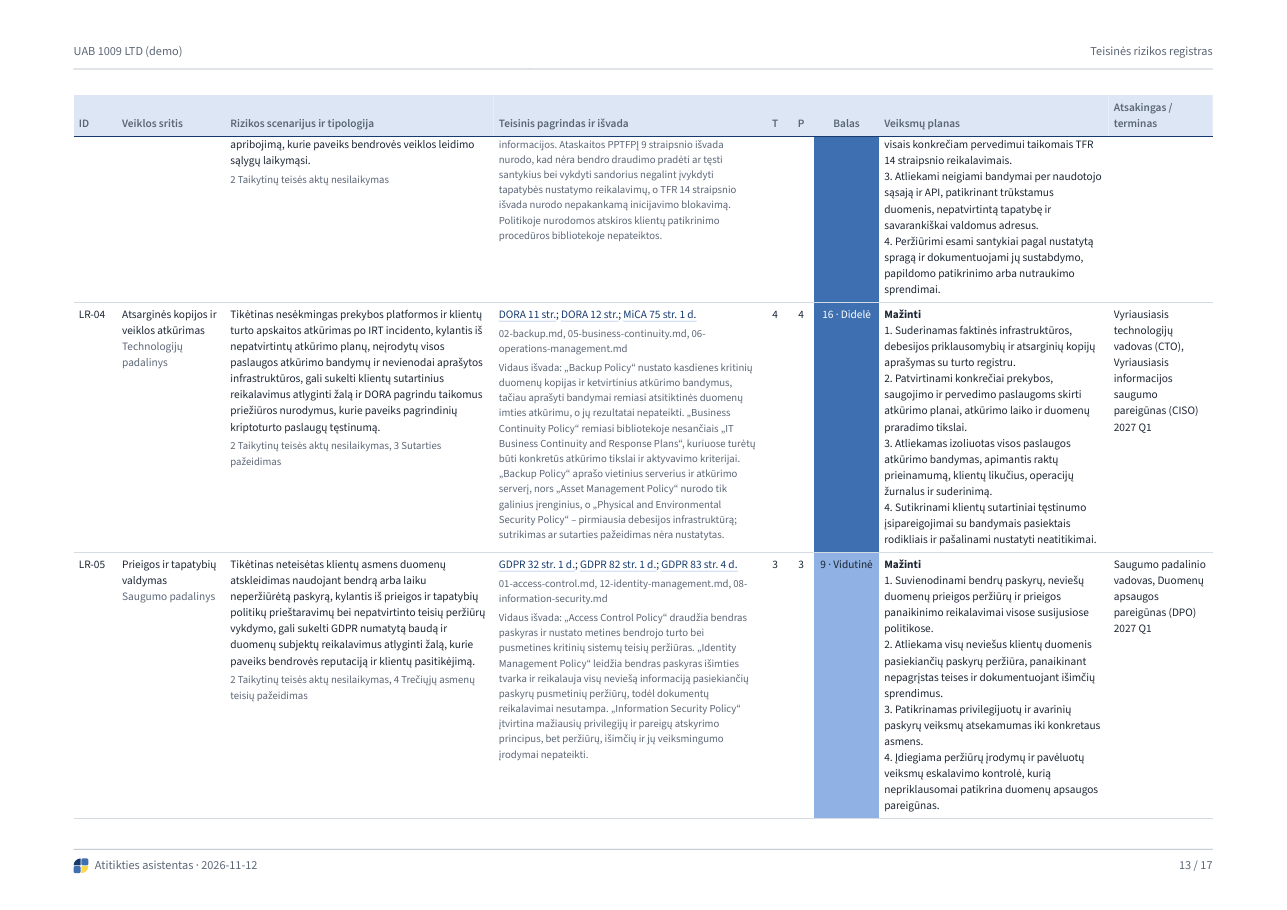
\includegraphics[width=\textwidth]{figures/samples/risks-register}
\caption{Teisinės rizikos registras, kaip jį pavyzdinei įmonei lietuvių kalba spausdina
sistemos PDF eksportas (13 puslapis iš 17; rizikos dokumentas sugeneruotas 2026 m. lapkričio
12~d. duomenų bazės kopijoje; gulsčias puslapis): vieno scenarijaus pabaiga ir du ištisi
scenarijai. Kiekvienoje eilutėje: id; veiklos sritis ir riziką valdantis padalinys; scenarijaus
sakinys su jo teisinės rizikos rūšimis; teisinis pagrindas, susiję dokumentai ir vidaus išvada;
tikimybė $T$, poveikis $P$ ir balas su rizikos lygiu, kuriuos apskaičiuoja kodas; reagavimo
būdas su veiksmais; atsakingi asmenys ir ketvirtis.}\label{fig:programme:registerpage}
\end{figure}

\subsection{Skaičiai apskaičiuojami, niekada neimami iš modelio}

Scenarijų schemoje nėra lauko nei tikimybės lygiui, nei poveikio lygiui, nei balui, nei
rizikos lygiui. Jei redaguotame turinyje tokių reikšmių yra, \code{validate} jas perrašo.
Aritmetika užima penkias eilutes.

% The box opens with a block of code, which cannot be split: room for both
\needspace{15\baselineskip}
\begin{codebox}{Scenarijaus aritmetika (\code{risks.validate}, \code{band_of})}
\begin{codeblock}
level = lambda value: value if isinstance(value, int) and not isinstance(value, bool) and 1 <= value <= 5 else 0

chance = {dimension: level((row.get("likelihood") or {}).get(dimension)) for dimension in LIKELIHOOD_DIMENSIONS}
harm = {dimension: level((row.get("impact") or {}).get(dimension)) for dimension in IMPACT_DIMENSIONS}
scored = all(chance.values()) and all(harm.values())
# The likelihood is the mean of its dimensions, halves up; the impact the gravest of its dimensions
t = int(sum(chance.values()) / len(chance) + 0.5) if scored else 0
p = max(harm.values()) if scored else 0
band = band_of(t * p) if scored else None
\end{codeblock}

\begin{codeblock}
def band_of(score):
    for band, (_, highest, *_rest) in BANDS.items():
        if score <= highest:
            return band
    return "critical"
\end{codeblock}

\begin{itemize}
  \item \textbf{Tikimybė} $T$: keturių tikimybės lygių vidurkis, suapvalintas (0,5 ---
        į didesnę pusę).
  \item \textbf{Poveikis} $P$: didžiausias iš keturių poveikio lygių. Viena katastrofinė
        pasekmė yra katastrofinis poveikis, kad ir kokie būtų kiti trys.
  \item \textbf{Balas}: $T \times P$. \textbf{Rizikos lygis}: pirmasis
        \cref{tab:programme:bands} rizikos lygis, kurio viršutinės ribos balas neviršija.
  \item \textbf{Id}: scenarijaus vieta sąraše, pavidalu \code{LR-01}, \code{LR-02}, …,
        numeruojama iš naujo kiekvieną kartą išsaugant.
  \item Lygis, kuris nėra sveikasis skaičius nuo 1 iki 5, laikomas nenustatytu. Scenarijus,
        kurio bent vienas lygis nenustatytas, turi $T = P = 0$, balą 0, neturi rizikos lygio
        ir pažeidžia taisyklę \code{scores}.
\end{itemize}

Pavyzdys iš modulio testo: tikimybės lygių 3, 2, 2, 3 vidurkis yra 2,5, todėl $T = 3$;
poveikio lygiai 2, 4, 3, 2 duoda $P = 4$; balas yra 12, rizikos lygis --- \code{medium}.
\end{codebox}

\begin{figure}[H]
\centering
\begin{tikzpicture}[x=14mm, y=9.5mm]
  \foreach \l in {1,...,5} {
    \foreach \p in {1,...,5} {
      \pgfmathtruncatemacro{\programmescore}{\l*\p}
      \ifnum\programmescore<4 \def\programmefill{tint}\def\programmetext{body}%
      \else\ifnum\programmescore<7 \def\programmefill{pale!45}\def\programmetext{body}%
      \else\ifnum\programmescore<13 \def\programmefill{pale}\def\programmetext{body}%
      \else\ifnum\programmescore<17 \def\programmefill{mid}\def\programmetext{white}%
      \else \def\programmefill{ink}\def\programmetext{white}%
      \fi\fi\fi\fi
      \path[fill=\programmefill, rounded corners=1.5pt] (\l-0.46,\p-0.44) rectangle (\l+0.46,\p+0.44);
      \node[text=\programmetext, font=\sffamily\small\bfseries] at (\l,\p) {\programmescore};
    }
  }
  \draw[ink, line width=1.3pt, rounded corners=1.5pt] (3-0.46,4-0.44) rectangle (3+0.46,4+0.44);
  \foreach \l/\name in {1/Labai mažai tikėtina, 2/Mažai tikėtina, 3/Vidutiniškai tikėtina, 4/Tikėtina, 5/Beveik neabejotina}
    \node[font=\sffamily\scriptsize, text=muted, text width=13mm, align=center, anchor=north] at (\l,0.5) {\textbf{\l}\\ \name};
  \foreach \p/\name in {1/Nereikšmingas, 2/Mažas, 3/Vidutinis, 4/Didelis, 5/Katastrofinis}
    \node[font=\sffamily\scriptsize, text=muted, anchor=east] at (0.45,\p) {\name\enspace\textbf{\p}};
  \node[font=\sffamily\scriptsize\bfseries, text=mid, anchor=north] at (3,-0.55) {TIKIMYBĖ $T$ (keturių aspektų vidurkis, suapvalintas)};
  \node[font=\sffamily\scriptsize\bfseries, text=mid, anchor=south, rotate=90] at (-1.45,3) {POVEIKIS $P$ (didžiausias iš keturių)};
  \foreach \i/\fillc/\name/\range in {5/ink/Kritinė/20--25, 4/mid/Didelė/15--16, 3/pale/Vidutinė/8--12, 2/pale!45/Toleruotina/4--6, 1/tint/Nereikšminga/1--3} {
    \path[fill=\fillc, rounded corners=1.5pt] (6.0,\i-0.25) rectangle (6.45,\i+0.25);
    \node[font=\sffamily\scriptsize, anchor=west] at (6.55,\i) {\textbf{\name}\enspace\range};
  }
\end{tikzpicture}
\caption{5×5 matrica ir jos penki rizikos lygiai. Kiekviename langelyje --- balas, kurį duoda
jo du lygiai. Dviejų lygių nuo 1 iki 5 sandaugos niekada nepatenka tarp rizikos lygių
intervalų. Išskirtas langelis --- tekste aptartas pavyzdys: $T = 3$, $P = 4$,
balas~12.}\label{fig:programme:matrix}
\end{figure}

Konsolė laikosi tos pačios taisyklės. Scenarijaus forma siunčia tik aštuonis lygius ir
\enquote{niekada neįrašo skaičiaus ten, kur žmogus jo nepasirinko}
(\file{pages/Programme/ScenarioEditor.jsx}); scenarijus, kurio lygiai pakeisti, bet dar
neišsaugoti, lygio nerodo ir į matricą neįtraukiamas, kol serveris neatsako. Pokalbių
asistentui liepiama registro skaičius cituoti ir niekada jų neperskaičiuoti bei nepriskirti
kitam rizikos lygiui (\cref{sec:programme:chat}). Vieno įvesties šaltinio balai neturi, ir tai
čia nurodoma kaip žinomas apribojimas: sankcijų pakopos, kurias sistema nuskaito iš teisės aktų
(\cref{ch:obligations}), poveikio lygių neveikia --- šie lieka modelio kriterijų
interpretacija.

\begin{figure}[H]
\centering
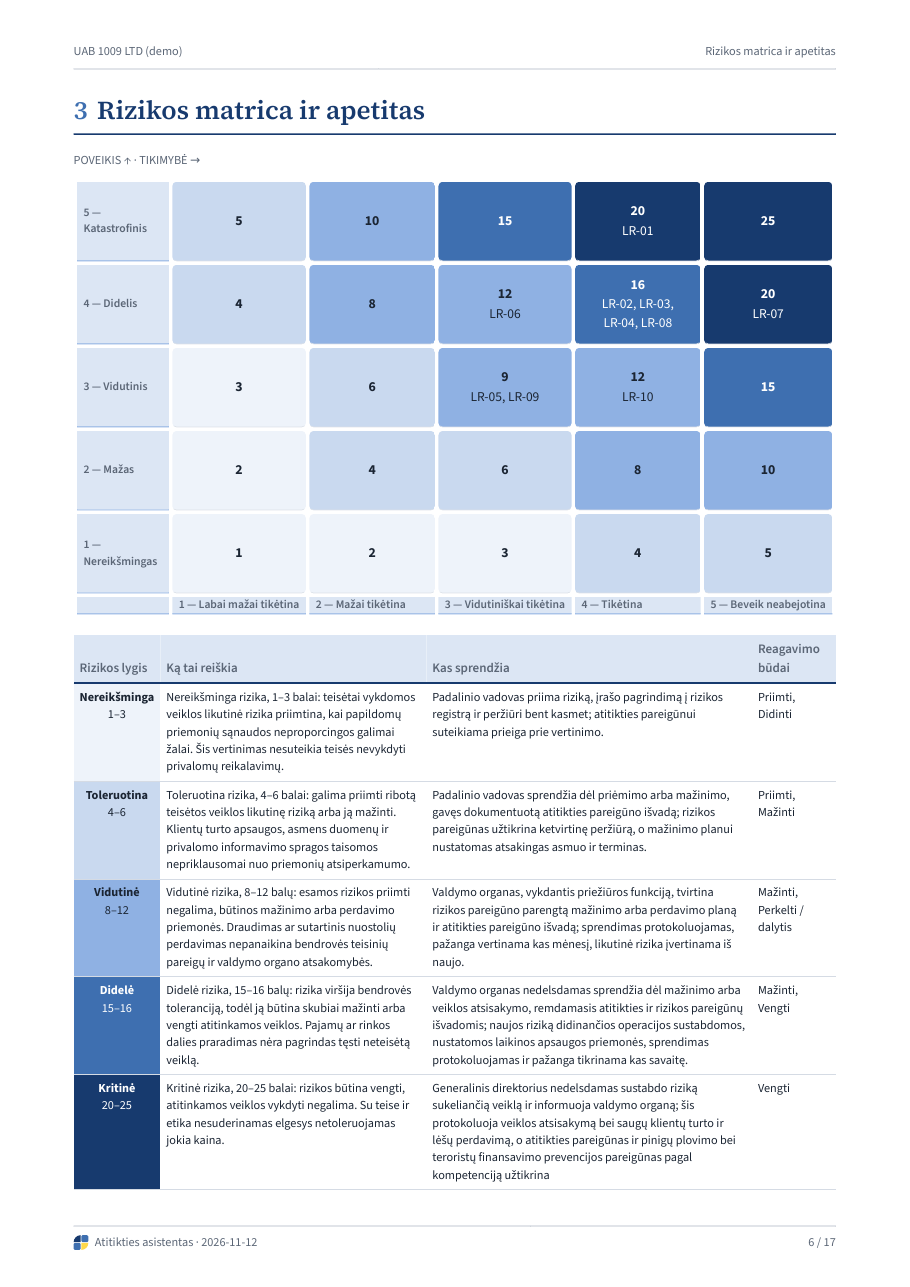
\includegraphics[width=.6\textwidth]{figures/samples/risks-matrix}
\caption{To paties registro matrica, kaip ją spausdina PDF eksportas (6 puslapis iš 17,
lietuvių kalba): poveikis --- aukštyn, tikimybė --- į dešinę, kiekviename langelyje balas ir į
jį patenkančių scenarijų id; iš dešimties du yra kritinio lygio, keturi --- didelio ir keturi
--- vidutinio. Apačioje --- penki dokumento kriterijų rizikos lygiai: ką kiekvienas reiškia,
kas sprendžia ir kokius reagavimo būdus jis leidžia.}\label{fig:programme:matrixpage}
\end{figure}

\subsection{Registro taisyklės}

\begin{xltabular}{\textwidth}{@{}L{37mm}L{17mm}Y@{}}
\caption{Taisyklės, kurias tikrina \code{risks.validate}, ta tvarka, kuria ji jas pateikia}\label{tab:programme:riskrules}\\
\toprule
\hd{Taisyklė} & \hd{Pobūdis} & \hd{Laikomasi, kai} \\
\midrule
\endfirsthead
\toprule
\hd{Taisyklė} & \hd{Pobūdis} & \hd{Laikomasi, kai} \\
\midrule
\endhead
\bottomrule
\endlastfoot
\code{criteria} & privaloma & Nė vienas iš keturiasdešimties abiejų kriterijų lentelių langelių nėra tuščias, rizikos apetite kiekvienas rizikos lygis turi savo komentarą ir sprendimą, o kriterijų pritaikymo paaiškinimas parašytas. Detalėse nurodomas tuščių vietų skaičius. \\
\code{scenarios} & privaloma & Yra bent \code{MIN_SCENARIOS}~=~5 scenarijai. \\
\code{categories} & privaloma & Visi scenarijai kartu nurodo bent \code{MIN_CATEGORIES}~=~4 iš šešių teisinės rizikos rūšių. \\
\code{sentence} & privaloma & Kiekvienas scenarijus turi sakinį ir visas keturias jo dalis: įvykį, šaltinį, pasekmes, tikslą. \\
\code{ties} & privaloma & Kiekvienas scenarijus nurodo padalinį ir bent vieną politiką, kuri yra įmonės dokumentas. \\
\code{scores} & privaloma & Kiekvienas scenarijus turi visus aštuonis lygius --- sveikuosius skaičius nuo 1 iki 5. \\
\code{provisions} & privaloma & Nė viena scenarijaus nurodyta nuostata neturi būsenos \code{not_found}. \\
\code{provisions_unverified} & įspėjimas & Nė viena nuostata nenurodo teisės akto, kurio bazėje nėra. \\
\code{provision_subjects} & įspėjimas & Nė viena nuostata nebuvo įvertinta kaip \code{mismatch}. \\
\code{owners} & įspėjimas & Kiekvienas scenarijus turi bent vieną atsakingą asmenį ir terminą. \\
\code{response_fit} & įspėjimas & Kiekvieno įvertinto scenarijaus reagavimo būdas yra vienas iš tų, kuriuos leidžia jo rizikos lygis. \\
\code{sentence_form} & įspėjimas & Kiekviename sakinyje, neatsižvelgiant į raidžių dydį, yra keturi jo kalbos jungiamieji žodžiai: lietuviškai \enquote{Tikėtin}, \enquote{kylan}, \enquote{gali sukelti}, \enquote{paveik}; angliškai \enquote{likely}, \enquote{arising from}, \enquote{may cause}, \enquote{affect}. \\
\end{xltabular}

Likusį darbą atlieka normalizavimas: scenarijus išlaiko daugiausia dvi rūšis --- tas dvi,
kurių jo nurodyti numeriai mažiausi; reagavimo būdas, nepatenkantis tarp penkių galimų, tampa
\code{mitigate}; politika, kuri nėra įmonės dokumentas, atmetama --- taip išgalvota nuoroda
baigiasi pažeista taisykle \code{ties}. Vienas laukas schemoje neturi atitikmens:
\code{externalConclusion}, išorės teisininko nuomonė, kurią scenarijaus formoje gali įrašyti
tik žmogus. O vienas laukas visai netikrinamas: vidaus išvada yra laisvas modelio tekstas apie
įmonę, su šaltiniais susietas tik nurodymu remtis įvesties faktais. Tai scenarijaus dalis,
kurią peržiūrėtojas turėtų perskaityti pirmiausia.

\begin{pathcard}{Teisinės rizikos scenarijai}{programme.risk_scenarios}
  \pcrow{Trigger}{To pačios užduoties etapas \code{scenarios}, iškart po etapo
    \code{criteria}.}
  \pcrow{Input}{Tas pats bendras blokas. Duomenys: dvi kriterijų lentelės, kaip jas parašė
    pirmasis iškvietimas; teisinės rizikos rūšys ir šaltinių, pasekmių bei tikslų
    tipologijos; valdymo struktūros mazgų, kurių rūšis yra \code{unit} arba \code{function},
    pavadinimai arba pastaba, kad struktūros dokumento nėra; rinkinys kaip nuorodos ir
    pavadinimai; iki 36 atvirų naujausios ataskaitos išvadų, rimčiausios pirmiau, kiekviena su
    220 analizės ženklų.}
  \pcrow{Prompt and model}{\prompt{programme.risk_scenarios}, 1~versija, modelis
    \model{gpt-6.1-sol}, temperatūra~0,3. Schema \code{SCENARIOS_SCHEMA}, pavadinimu
    \code{risk_scenarios}. \enquote{Kantrus} iškvietimas.}
  \pcrow{Output}{\code{title}; \code{scenarios[]}: \code{area}, \code{unit},
    \code{sentence}, \code{event}, \code{source}, \code{consequences}, \code{objective},
    \code{categories[]} (1--6), \code{sourceType} (1--6), \code{consequenceType} (1--5),
    \code{objectiveType} (1--5), \code{legalBasis[]}, \code{policyRefs[]},
    \code{internalConclusion}, \code{likelihood} (keturi lygiai 1--5 ir \code{why}),
    \code{impact} (keturi lygiai 1--5 ir \code{why}), \code{response} (\code{accept},
    \code{increase}, \code{mitigate}, \code{transfer}, \code{avoid}), \code{actions[]},
    \code{owners[]}, \code{deadline}.}
  \pcrow{Checked by code}{Priskiriami id; apskaičiuojami tikimybė, poveikis, balas ir rizikos
    lygis; politikų nuorodos paverčiamos įmonės dokumentais; nuostatos ieškomos ir vieną
    kartą įvertinamos; tikrinamos dvylika taisyklių (\cref{tab:programme:riskrules}).}
  \pcrow{Stored}{\code{work_products.content} (\code{title}, \code{scenarios}).}
  \pcrow{On failure}{Nekartojama; pirmojo iškvietimo kriterijai prarandami kartu su
    generavimu.}
  \pcrow{Cost}{Generavimą pradėjęs naudotojas; tai dalis nuo 0,35 iki 0,48~\$, išmatuotų už
    dokumentą.}
  \pcrow{Human control}{Žmogus redaguoja scenarijaus laukus, įskaitant aštuonis lygius ir
    scenarijaus vietą trijose tipologijose, prideda ar šalina scenarijus, gali
    įrašyti išorės teisininko išvadą ir patvirtina registrą. Modelio nurodyti lygiai yra
    projektas, kurį peržiūrėtojas taiso.}
  \pcrow{Measured by}{Pačios instrukcijos niekas nematuoja. Du trūkumai, pastebėti pirmuosiuose
    jos registruose, lėmė toliau aprašytus pakeitimus.}
\end{pathcard}

\subsection{Dvi pirmųjų registrų pamokos}

Scenarijų instrukcija dabartinę formuluotę įgavo po dviejų pastebėjimų su pavyzdine įmone,
užfiksuotų faile \file{docs/markdown/en/architecture.md}. Nė vieno iš šių trūkumų rūšies taisyklė negali
aptikti: jokia taisyklė nežiūri, kaip pasiskirsto balai ar su kuriomis politikomis susiję
scenarijai.

\begin{lessonbox}{2026 m. lapkričio 12 d.: vienodi poveikio vertinimai}
Pirmasis \demo{} sugeneruotas registras devyniems iš dešimties scenarijų priskyrė tuos pačius
poveikio lygius --- \enquote{bauda, licencijos praradimas nepreziumuojamas} --- ir niekur
neįvertino abejonės dėl paties leidimo apimties. Instrukcija buvo pakeista: modeliui liepiama
kiekvieną scenarijų vertinti pagal jo paties faktus ir pirmiausia iškelti rizikas, dėl kurių
įmonė galėtų netekti leidimo, klientų turto ar pagrindinės paslaugos tęstinumo. Antrojo
registro balai pasiskirstė nuo 9 iki 20. (Instrukcija taip pat liepia modeliui vertinti
pagrįstai numatomą rimtą atvejį ir nurodyti, kurį atvejį jis vertino; žr. ištrauką aukščiau.)
\end{lessonbox}

\begin{lessonbox}{2026 m. lapkričio 12 d.: scenarijai, susieti su finansų politikomis}
Antrasis registras savo scenarijus siejo vien su finansų politikomis, o kurso užduotis
scenarijus sieja su technologijų, operacijų ir saugumo padaliniais ir jų politikomis. Dabar
instrukcija tai sako žodžiais:

\begin{promptexcerpt}{programme.risk_scenarios}{aprėpti visą organizaciją}
[…]
Cover the organisation, not one corner of it: where the company has units for technology, for operations and for security, each of them owns at least one scenario, and at least a third of the scenarios turn on its operational and information-security policies (access control, backup, business continuity, operations, assets, incidents, suppliers) – legal risk arises there too: a contract breached when a restore fails, personal data lost through access nobody reviewed, a right against a supplier never used.
\end{promptexcerpt}

Trečiasis registras turėjo dešimt scenarijų, apimančių visas šešias teisinės rizikos rūšis ir
šešis padalinius, o tarp septyniolikos dokumentų, su kuriais jie susiję, buvo septynios
informacinių technologijų politikos.
\end{lessonbox}


% ------------------------------------------------------------
\section{Žmogaus eilė: redagavimas, patvirtinimas, naujos versijos}\label{sec:programme:person}

Sugeneruotas dokumentas yra projektas atskirame konsolės puslapyje
(\file{pages/Programme/ProductPage.jsx}). Virš turinio yra skydelis \ui{Taisyklės}: sakinys,
kiek privalomų taisyklių pažeista arba kad nepažeista nė viena, ir kiekviena rūšies taisyklė
su jos būsena --- \ui{laikomasi}, \ui{pažeista} arba \ui{pastaba} --- ir detalėmis, kas ją
pažeidė. Žemiau turinys rodomas rūšies skiltyse (\cref{tab:programme:tabs}); paskutinė
kiekvienos rūšies skiltis, \ui{Kilmė}, išvardija, ką generavimas skaitė, kokios instrukcijų
versijos ir modeliai jį parengė ir kiek jis kainavo.

\begin{table}[H]
\caption{Dokumento puslapio skiltys ir ką žmogus gali keisti projekte}\label{tab:programme:tabs}
\begin{tabularx}{\textwidth}{@{}L{20mm}L{38mm}Y@{}}
\toprule
\hd{Rūšis} & \hd{Skiltis} & \hd{Ką galima redaguoti projekte} \\
\midrule
\code{policy} & \ui{Politika} & Kiekvienos dalies tekstą, sprendimus ir teisinį pagrindą; antraštės nustatytos. \\
 & \ui{Dokumentai} & Kiekvieno dokumento lygmenį ir temą; kiekvieno trūkstamo dokumento pavadinimą, paskirtį, lygmenį, prioritetą ir nuostatas arba jį pašalinti. \\
\code{governance} & \ui{Struktūra} & Mazgus: pavadinimą, rūšį, liniją, tėvinį mazgą, žymą \enquote{siūloma}, pastabą; mazgus pridėti ir šalinti. \\
 & \ui{Procesas ir RACI} & Etapus su jų pagrindu; kiekvieną matricos langelį; pridėti rolę kaip stulpelį. \\
 & \ui{Pareigybės ir spragos} & Nieko: tai įrašas apie tai, ką rado generavimas. \\
\code{risks} & \ui{Registras} & Scenarijaus laukus, įskaitant aštuonis lygius, bet ne jo šaltinio, pasekmės ir tikslo rūšis; scenarijus pridėti ir šalinti. \\
 & \ui{Kriterijai} & Kiekvieno langelio formuluotę, kalibravimo pastabą, kiekvieno rizikos lygio reikšmę ir sprendimą. \\
\bottomrule
\end{tabularx}
\end{table}

\subsection{Pakeitimas pereina tą pačią patikrą}

\ui{Redaguoti} turinį paverčia formomis. Pakeitimai lieka puslapyje, kol žmogus juos išsaugo;
išsaugant visas turinys siunčiamas maršrutu \route{PUT}{/api/programme/{id}/content}. Rodinys
\code{product_content} atmeta viską, kas nėra projektas (409 \code{NOT_DRAFT}), ir kviečia tą
pačią \code{validate}, kurią kvietė generavimas, tik be argumento \code{judge}, \ie be modelio:
citatos vėl ieškomos, nuostatos vėl tikrinamos, lygiai, balai, rizikos lygiai ir id vėl
apskaičiuojami, o kiekviena taisyklė vėl patikrinama. Išsaugomas ir atsakyme grąžinamas
normalizuotas turinys su naujomis patikromis, redaguotojo vardu ir laiku. Puslapis savo kopiją
pakeičia atsakymu, todėl tai, kas po išsaugojimo matoma ekrane, yra tai, ką laiko serveris, su
kiekviena taisykle, kurią pakeitimas pataisė ar pažeidė.

Taigi žmogui ir modeliui taikomos tos pačios taisyklės, tikrinamos to paties kodo. Žmogus gali
projektą pataisyti --- pašalinti nuostatą, kurios teisės akte nėra, suteikti etapui atskaitingą
rolę --- ir gali jį sugadinti: pakeitimas, po kurio etapas turi dvi atskaitingas roles,
padaro projektą nepatvirtinamą, kol jis nepataisomas.

\subsection{Patvirtinimas užšaldo dokumentą}

\ui{Patvirtinti} atveria dialogą, kuris paaiškina, ką reiškia patvirtinimas, ir leidžia
įrašyti neprivalomą pastabą. Užklausa yra
\route{PATCH}{/api/programme/{id}} su \code{approved: true}. Rodinys \code{product_item} ją
priima tik projektui ir tik tada, kai nepažeista nė viena privaloma taisyklė; kitaip jis atsako
409 \code{RULES_BROKEN} ir įvardija taisykles. Puslapis mygtuką išjungia iš anksto ir nurodo
priežastį, kol pažeista privaloma taisyklė arba projekte yra neišsaugotų pakeitimų.
Patvirtinimas įrašo, kas patvirtino, kada, ir pastabą (daugiausia 2\,000 ženklų), o veiksmų
žurnale registruojamas kaip \code{programme.approve}. Patvirtinti gali bet kuris įmonę matantis
naudotojas --- jos savininkas ar administratorius; pokalbių asistentas tam įrankio neturi.

Patvirtinto dokumento redaguoti negalima: \code{PUT} jį atmeta. \ui{Nauja versija} siunčia
\route{POST}{/api/programme/{id}/revise}: patvirtintas turinys ir jo patikros nukopijuojami į
naują projektą su kitu versijos numeriu ir \code{revisedFrom} jo pagrinde; patvirtinta versija
lieka tokia, kokia buvo patvirtinta. Maršrutas atsisako, kai naujesnė tos rūšies versija jau
laukia eilėje, generuojama arba yra projektas (409 \code{NEWER_VERSION}). Taip sukurtas
projektas neturi savo generavimo, todėl jo kilmė nerodo nei instrukcijų, nei kainos.

\begin{figure}[H]
\centering
\begin{tikzpicture}[node distance=15mm and 19mm]
  \node[svc, minimum width=19mm] (queued) {eilėje};
  \node[ai, minimum width=19mm, right=of queued] (running) {generuojama};
  \node[chk, minimum width=19mm, right=of running] (draft) {projektas\\ {\scriptsize $n$ versija}};
  \node[man, minimum width=19mm, right=of draft] (approved) {patvirtinta\\ {\scriptsize užšaldyta}};
  \node[svc, minimum width=19mm, below=of queued] (cancelled) {atšaukta};
  \node[svc, minimum width=19mm, below=of running] (failed) {nepavyko};
  \node[chk, minimum width=19mm, below=of approved] (next) {projektas\\ {\scriptsize $n{+}1$ versija}};
  \draw[flow] (queued) -- node[lbl, above, align=center] {vykdytojas\\ paima užduotį} (running);
  \draw[flow] (running) -- node[lbl, above, align=center] {taisyklės\\ patikrinamos} (draft);
  \draw[flow] (draft) -- node[lbl, above, align=center] {žmogus\\ patvirtina} node[lbl, below, align=center] {nepažeista nė\\ viena privaloma} (approved);
  \draw[flow] (queued) -- node[lbl, left, align=right] {žmogus\\ sustabdo} (cancelled);
  \draw[flow] (running) -- (cancelled);
  \draw[flow] (running) -- node[lbl, right, align=left] {klaida arba\\ vykdytojas nutrūko} (failed);
  \draw[flow] (approved) -- node[lbl, left, align=right] {žmogus kuria naują\\ versiją: kopija} (next);
  \draw[flow] (draft.south west) .. controls +(-5mm,-9mm) and +(5mm,-9mm) .. node[lbl, below, align=center] {žmogus išsaugo pakeitimą:\\ vėl patikrinama, be modelio} (draft.south east);
\end{tikzpicture}
\actorlegend
\caption{Vienos programos dokumento versijos būsenos. Būsenos spalva rodo, kas ją sukuria: kol
versija yra \code{running}, vyksta modelio iškvietimai; \code{draft} patikrino kodas, o
\code{approved} ją padaro tik žmogus. Bet kurios būsenos, išskyrus \code{queued} ir
\code{running}, versiją galima ištrinti.}\label{fig:programme:states}
\end{figure}

\subsection{Sustabdymas ir trynimas}

\ui{Stabdyti generavimą} siunčia \route{POST}{/api/programme/{id}/cancel}. Eilėje laukianti
užduotis atšaukiama iš karto; vykdoma pažymima ir sustoja prieš kitą modelio iškvietimą, todėl
jau pradėtas iškvietimas baigiamas ir už jį sumokama. Versiją, kuri nelaukia eilėje ir nėra
generuojama, galima ištrinti per \route{DELETE}{/api/programme/{id}} --- taip pat ir patvirtintą;
kitos versijos lieka. Dokumento sukūrimas, redagavimas, patvirtinimas, naujos versijos kūrimas,
atšaukimas, trynimas ir eksportas --- kiekvienas įrašo veiksmų žurnalo įrašą
(\cref{ch:security}).


% ------------------------------------------------------------
\section{Struktūros schema ir eksportas}\label{sec:programme:outputs}

\subsection{Vienas brėžinys puslapiui ir popieriui}

Valdymo struktūros dokumento struktūrą nubraižo API, ne konsolė: \code{structure_svg} faile
\file{programme/chart.py} mazgus paverčia vienu SVG paveikslu, kurį
\route{GET}{/api/programme/{id}/chart} pateikia puslapiui ir kuris įterpiamas į PDF. Todėl
puslapis ir popierius negali skirtis. Konsolė paveikslą atsisiunčia kaip failą ir rodo
paveikslo elemente; SVG žymėjimas į puslapį niekada neįterpiamas, o kiekvienas jame esantis
tekstas ekranuojamas.

Kiekvienas mazgas yra 180 × 66 vienetų stačiakampis po savo tėviniu mazgu, su pavadinimu
daugiausia trijose eilutėse po 23 ženklus. Stačiakampis nuspalvinamas pagal liniją ---
valdymo organai tamsiai mėlyna prekės ženklo spalva, pirmoji linija šviesia, antroji apvesta
mėlynai, trečioji pažymėta geltonai, išorės užtikrinimas pilkai --- o siūlomas mazgas
brėžiamas punktyriniu kontūru su žodžiu \enquote{siūloma}. Po medžiu esanti legenda spalvas
pakartoja žodžiais. Išdėstymas --- kaip organizacinės schemos: viršutiniai medžio lygiai
išskleidžiami eilėmis, mazgo vaikiniai mazgai rikiuojami pagal liniją, kad trys linijos būtų skaitomos
iš kairės į dešinę; vaikiniai mazgai, po kuriais nieko nėra, neužima po atskirą stulpelį, o kabo kartu,
iki penkių ant vieno bėgelio (\code{RAIL}); gilesni lygiai sudedami po savo tėviniu mazgu, su
įtrauka kiekvienam lygiui. Kiek lygių išskleidžiama eilėmis --- vienas, du ar trys ---
parenkama taip, kad brėžinys geriausiai tilptų į gulsčio puslapio 263 × 148 laukelį
(\code{PAGE_W}, \code{PAGE_H}).

\begin{figure}[H]
\centering
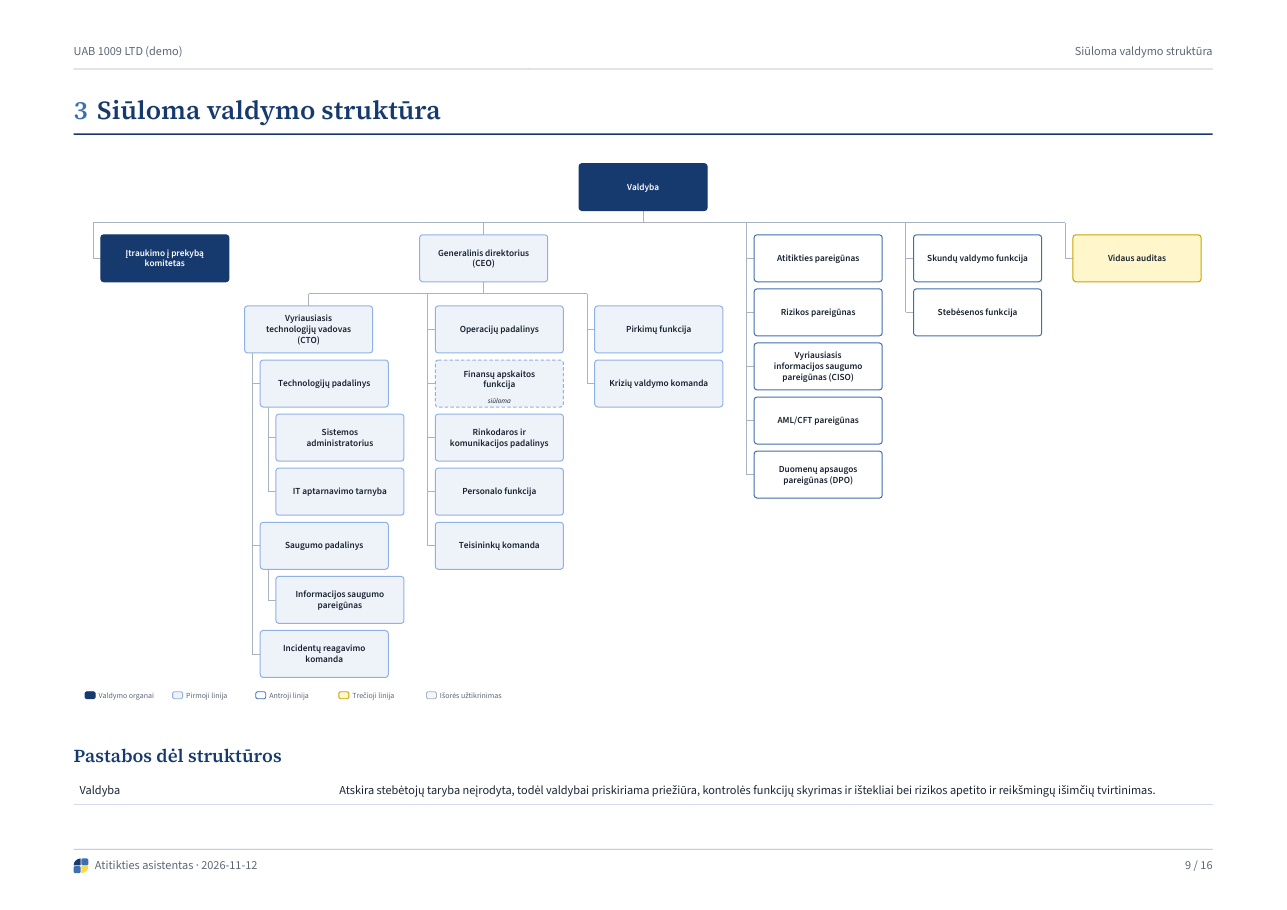
\includegraphics[width=\textwidth]{figures/samples/governance-chart}
\caption{Siūloma struktūra, kaip ją spausdina PDF eksportas (9 puslapis iš 16; valdymo
struktūros dokumentas tas pats kaip \cref{fig:programme:racipage}; gulsčias puslapis): tas pats
paveikslas, kurį rodo konsolė. Valdymo organai tamsiai mėlyni --- valdyba ir komitetas; pirmoji
linija šviesiuose stačiakampiuose po vadovu; antroji linija apvesta mėlynai; vidaus auditas,
trečioji linija, pažymėtas geltonai; modelio siūloma finansų funkcija --- punktyrinė ir pažymėta
\enquote{siūloma}; po medžiu legenda. Žemiau prasideda pastabos dėl
struktūros.}\label{fig:programme:chartpage}
\end{figure}

\subsection{Eksportas}

\route{GET}{/api/programme/{id}/export?format=} projektą ar patvirtintą dokumentą perduoda kaip
failą (\file{programme/exports.py}); kitos būsenos dokumentas neturi ko eksportuoti.

\begin{table}[H]
\caption{Kiekvienos rūšies eksporto formatai (\code{FORMATS})}\label{tab:programme:exports}
\begin{tabularx}{\textwidth}{@{}L{20mm}L{13mm}Y@{}}
\toprule
\hd{Rūšis} & \hd{Formatas} & \hd{Ką failas apima} \\
\midrule
visos & PDF & Viršelis; turinys; dokumentas sunumeruotais skirsniais; paskutinis skirsnis, \enquote{Patikros ir kilmė}, su kiekviena taisykle, kaip dokumentas jos laikėsi ar ją pažeidė, ir iš ko jis parengtas. \\
\code{policy} & Word & Pavadinimas, įmonė, versija ir ar tai projektas; aštuonios dalys su sunumeruotomis antraštėmis; valdymo organui palikti klausimai, surinkti pabaigoje. \\
\code{risks} & Excel & Keturi lapai: registras keturiolikoje stulpelių, tikimybės kriterijai, poveikio kriterijai ir rizikos lygiai su jų reikšme, sprendimu ir reagavimo būdais. \\
\bottomrule
\end{tabularx}
\end{table}

PDF parengiamas su ataskaitos stilių lentele, šriftais ir puslapio apipavidalinimu
(\file{analysis/pdf.py}, \cref{ch:report}), todėl įmonės ataskaita ir jos programa skaitomos
kaip vienas rinkinys. Viršelyje nurodoma rūšis, pavadinimas, įmonė, data ir versija, taip pat arba
kas ir kada dokumentą patvirtino, arba \enquote{Projektas --- žmogaus dar nepatvirtintas}.
Politikos skirsniai yra jos aštuonios dalys --- kiekviena su atvirais sprendimais išskirtame
laukelyje, dokumentais, kuriais ji remiasi, ir teisiniu pagrindu kaip nuorodomis į oficialų
tekstą, --- o po jų eina hierarchija ir trūkstami dokumentai, kiekvienas su politikos dalimi,
kuriai jis skirtas. Valdymo struktūros PDF schemą ir
RACI matricą pateikia gulsčiuose puslapiuose: matricoje rolių pavadinimai eina stulpeliais
aukštyn, o atskaitingo langelis užlietas tamsiai mėlyna. Rizikos PDF pateikia dvi kriterijų
lenteles, matricą su kiekvieno scenarijaus id tame langelyje, į kurį jį patalpina jo lygiai,
po jos rizikos lygių lentelę, scenarijus po vieną --- kiekvieną su jo teisinės rizikos
rūšimis ir vieta trijose tipologijose --- ir registrą gulsčiame puslapyje devyniais
stulpeliais.

Kiti du formatai egzistuoja dėl to, ką su dokumentais daroma toliau. Valdyba politiką prieš
priimdama redaguoja --- todėl Word failas; registras saugomas ir su juo dirbama --- todėl
darbaknygė. Darbaknygėje kiekvienas langelis įrašomas kaip tekstas ar skaičius, todėl joks
dokumento tekstas negali tapti formule.


% ------------------------------------------------------------
\section{Ką pokalbis gali ir ko negali}\label{sec:programme:chat}

Pokalbių asistentas (\cref{ch:chat}) programos dokumentus pasiekia dviem įrankiais, kurie
apibrėžti asistento paslaugos faile \file{llm/tools/programme.js} ir išvardyti kartu su visais
kitais įrankiais (\cref{app:tools}).

\begin{table}[H]
\caption{Du pokalbio įrankiai programos dokumentams}\label{tab:programme:chat}
\begin{tabularx}{\textwidth}{@{}L{34mm}Y@{}}
\toprule
\hd{Įrankis} & \hd{Ką daro} \\
\midrule
\code{startWorkProduct} & Kviečia tą patį maršrutą kaip konsolės mygtukas, su rūšimi ir kalba. API atsisakymas --- nėra dokumentų, vienas jau generuojamas, biudžetas išnaudotas --- grįžta ne kaip klaida, o kaip atsakymas, kuris pasako, ką daryti toliau. \\
\code{getWorkProduct} & Vien su įmone: naujausia kiekvienos rūšies versija ir jos būsena. Su rūšimi ar dokumento id: tas dokumentas, perkurtas į glaustą pavidalą. Su \code{section}: tik registro kriterijų lentelės arba tik valdymo struktūros dokumento pareigybės. \\
\bottomrule
\end{tabularx}
\end{table}

Dokumento turinys, kaip jį laiko API, užima apie 80~kB, ir jis niekada neperduodamas modeliui
visas. \code{getWorkProduct} jį perkuria: nuostata tampa viena eilute su žyma, kur paieška
įspėja, citata --- jos dokumento pavadinimu, struktūra --- įtraukomis išdėstytu planu, matrica
--- po eilutę kiekvienam etapui su rolėmis, nurodytomis pavadinimais. Taisyklės, kurių
dokumentas nesilaiko, pateikiamos žodžiais, privalomos --- atskirai nuo pastabų. Kiekviename
atsakyme apie dokumentą yra jo puslapio adresas.

Pokalbis negali nei redaguoti, nei patvirtinti dokumento; nė vienam iš šių veiksmų įrankio
nėra. Instrukcija \prompt{chat.assistant} šią ribą nubrėžia savo taisyklėje dėl programos
dokumentų:

\begin{promptexcerpt}{chat.assistant}{12 taisyklė, dėl programos dokumentų}
[…]
When there is none, offer to generate it: it works in the background for about five minutes and takes about 0.5 USD of today's budget – startWorkProduct only after the user's yes, the policy first, then the structure, then the register, since each builds on the ones before it. While one is being generated say so and go on. Never write such a document yourself in the chat in place of the product, and never call one approved: only a person approves, on its page.
\end{promptexcerpt}

Paskutinio sakinio priežastis --- tas skirtumas, apie kurį ir yra šis skyrius. Politika, kurią
pokalbis parašytų tiesiai į pokalbį, nebūtų perėjusi jokios taisyklės, nesiremtų nei surasta
citata, nei patikrinta nuostata ir neturėtų nei versijos, nei tvirtintojo.


% ------------------------------------------------------------
\section{Kaina ir matavimai}\label{sec:programme:cost}

Visos šešios instrukcijos veikia su \model{gpt-6.1-sol}, kurį DI tinklų sąsajos 2026 m.
lapkričio 10~d. kainoraštis įkainoja 2~\$ už milijoną įvesties žetonų, 10~\$ už milijoną
išvesties žetonų, 0,10~\$ --- už iš podėlio nuskaitytą įvestį ir 2,50~\$ --- už į podėlį
įrašytą įvestį. Generavimas --- tai du iškvietimai su tuo pačiu dokumentų rinkiniu: pirmasis
įrašo bendrą bloką į tiekėjo podėlį, antrasis jį iš ten nuskaito (\cref{ch:models}).

Biudžetas tikrinamas vieną kartą, pradžioje: naudotojui turi būti likę bent 0,25~\$ dienos biudžeto.
Prasidėjusio generavimo dienos biudžetas nesustabdo. Du rūšies iškvietimai ir bet kuris
inventorius įrašomi generavimą pradėjusiam naudotojui. Nuorodų vertintojo iškvietimas etape
\code{references} įrašomas užduoties etapui be naudotojo: jis įeina į kainą, kurią dokumentas
rodo kilmės skiltyje (ji sumuoja visus užduoties iškvietimus), bet ne į kurio nors naudotojo
dienos biudžetą. Prieš pradėdama konsolė naudotojui praneša, kad generavimas trunka apie
penkias minutes ir kainuoja apie 0,50~\$ (\code{RUN_COST_USD} faile
\file{pages/Companies/CompanyProgramme.jsx}); pokalbio įrankio aprašyme nurodoma nuo keturių iki šešių
minučių.

\begin{lessonbox}{Išmatuota 2026 m. lapkričio 12 d.}
Duomenų bazės kopijoje \demo{} buvo sugeneruota po vieną kiekvienos rūšies dokumentą su
\model{gpt-6.1-sol} (\file{docs/markdown/en/architecture.md}):

\begin{tabularx}{\linewidth}{@{}L{24mm}L{22mm}Y@{}}
\toprule
\hd{Rūšis} & \hd{Kaina} & \hd{Kas gauta} \\
\midrule
\code{policy} & 0,46~\$, penkios minutės & Aštuonios dalys; surastos 23 iš 23 citatų; rastos 24 iš 24 nuostatų; 16 trūkstamų dokumentų. \\
\code{governance} & 0,39~\$ & 46 pareigybės, 15 spragų, 25 mazgai, 14 etapų; auksinės taisyklės laikomasi; vienas įspėjimas --- atitikties pareigūnas dalyvauja kiekviename etape. \\
\code{risks} & nuo 0,35 iki 0,48~\$ & Dešimt scenarijų, apimančių visas šešias teisinės rizikos rūšis ir šešis padalinius; visų taisyklių laikomasi. \\
\bottomrule
\end{tabularx}

\smallskip
Tai vienos įmonės generavimai vieną dieną. Jie rodo, kad taisyklių laikytis įmanoma, bet ne
tai, kaip dažnai jų laikomasi.

Veikiančioje sistemoje 2026 m. lapkričio 13~d. \demo{} vėl buvo sugeneruota po vieną kiekvienos
rūšies dokumentą: politika už 0,51~\$ per penkias minutes, visų taisyklių laikomasi; valdymo
struktūra, procesas ir RACI už 0,53~\$ per šešias su puse minutės, keturiolika etapų, visų
taisyklių laikomasi; registras už 0,49~\$ per penkias su puse minutės, dešimt scenarijų,
apimančių penkias iš šešių teisinės rizikos rūšių, su dviem įspėjimais, kurie netrukdo
patvirtinti, --- teisiniu pagrindu Civiliniame kodekse, kurio teisės aktų bazėje nėra, ir viena
MiCA nuostata, kuri, nuorodų vertintojo nuomone, reglamentuoja ką kita. Visi trys yra projektai: nė
vieno žmogus nepatvirtino.
\end{lessonbox}


% ------------------------------------------------------------
\section{Kaip žinoma, kad tai veikia}\label{sec:programme:evaluation}

Šių šešių instrukcijų nematuoja joks vertinimo rinkinys. Sistemos turimi rinkiniai
(\cref{ch:control}) apima pareigų registro vertintoją, apimties skaitymą, nuorodų vertintoją,
atitikties spragų analizę, taikytinumą ir sankcijas; nė vienas negeneruoja programos dokumento
ir nelygina jo su laukiamu. Projekto kokybė užtikrinama dviem kitais būdais.

\begin{description}
  \item[Kodas, pagal taisykles.] Kiekvienas projektas, kad ir kas jį parašė, pereina
    \code{validate}. Taisyklės nustato, kad dokumentas išsamus, kad jo struktūra ir matrica
    tinkamai sudarytos, kad jo skaičiai išplaukia iš jo lygių ir kad jo nuorodos egzistuoja.
    \file{tests/test_programme.py} šį kodą testuoja su modelio imitacija: kad politika
    sukuriama kaip projektas su patikrintomis taisyklėmis, kad žmogus gali ją pataisyti,
    patvirtinti ir sukurti naują versiją, kad auksinė taisyklė ir linijų nepriklausomumas
    užtikrinami, kad nė vienas lygis, balas ar rizikos lygis nepriimamas aklai, kad kiekvienas
    galimas balas patenka į kurį nors rizikos lygį ir kad eksportas bei schema sukuriami. Šie
    testai nieko nepasako apie tai, ką rašo tikrasis modelis.
  \item[Žmogus, pagal savo vertinimą.] Ar politika tinka įmonei, ar rolės tikrai trūksta, ar
    RACI paskyrimas protingas, ar scenarijaus vidaus išvada teisinga ir jo lygiai tinkami ---
    nė vieno iš šių klausimų nesprendžia jokia taisyklė. Juos sprendžia dokumentą tvirtinantis
    žmogus, o sistema įrašo, kas tai buvo.
\end{description}

Dvi pamokos (\cref{sec:programme:risks}) rodo, kodėl antrasis būdas svarbus: nė vieno iš tų
trūkumų jokia taisyklė nebūtų pagavusi. Kol nėra etaloninių dokumentų rinkinio, patvirtintas
programos dokumentas yra tiek patikimas, kiek atidžiai jį perskaitė peržiūrėtojas; projektas
yra atspirties taškas, ir kiekvieno PDF viršelis pasako, kurį iš šių dviejų skaitytojas laiko
rankose.

Čia priklauso dar du apribojimai. Sistema nerengia nei metinės atitikties ataskaitos, nei
stebėsenos programos: trys rūšys --- tai viskas, ką ji parengia. O dokumentų rinkiniui,
didesniam nei 600\,000 ženklų, programos dokumento parengti apskritai negalima, nes generavimas
atsisako dirbti iš ištraukų (\cref{sec:programme:library}).
